% ======================================================================
%  FYS4480/FYS9480  Quantum mechanics for many-particle systems
%  Week 46, November 12-13, 2026
%  Lecture slides (Beamer).  Thursday: 2 x 45 min,  Friday: 2 x 45 min.
%
%  Thursday (double lecture): the linked-diagram theorem.  The wave operator
%  drawn -- linked, disconnected-but-linked and unlinked open diagrams at
%  second and third order -- and how closing them gives connected and unlinked
%  energy diagrams; the renormalisation terms as unlinked diagrams with a
%  minus sign; fourth order with normal-ordered vertices and the factorisation
%  of denominators; the theorem and its imaginary-time proof (chapter 9,
%  sections 9.15.7-9.15.9); exclusion-principle-violating diagrams; the
%  two-level benchmark.  These frames were originally Friday, lecture 4 of
%  week45.tex (moved here 2026-11-04) plus new material.
%  Friday: coupled-cluster theory, chapter 10, sections 10.1-10.7: the
%  exponential ansatz, the similarity-transformed Hamiltonian, termination,
%  the CCD equations, coupled cluster as a resummation, the pairing model.
%  Answers to the week-45 exercises (Exercises/ExercisesWeek45.tex) and the
%  week-46 exercises are on the last frames.
%  Companion notebook: week46.ipynb (numpy only; diagrams.py machinery, the
%  unlinked pieces, two copies, the two-level count, a CCD solver).
%  Diagram styles (pline, hline, vint, vtx, fvtx, hloop, fcidiagram) are
%  those of book.tex, so the chapter TikZ figures compile unchanged.
%
%  Reviewed November 4, 2026 (week46_reviewed.tex, merged 2026-11-05).
%  Build: pdflatex week46.tex (twice).
%  All diagrams and recomputed plot data are embedded; no external figures needed.
% ======================================================================
\documentclass[aspectratio=169,10pt]{beamer}

% ---------------------------------------------------------------- packages
\usepackage[utf8]{inputenc}
\usepackage[T1]{fontenc}
\usepackage{lmodern}
\usepackage{amsmath,amssymb,bm,mathtools}
\usepackage{booktabs}
\usepackage[most]{tcolorbox}
\usepackage{listings}
\usepackage{hyperref}
\usepackage{tikz}
\usepackage{pgfplots}\pgfplotsset{compat=1.18}
\usetikzlibrary{positioning,arrows.meta,decorations.markings,shapes.misc}
\usetikzlibrary{tikzmark}

% ---------------------------------------------------------------- look
\usetheme{default}
\useinnertheme{rectangles}
\setbeamertemplate{navigation symbols}{}
\definecolor{uioblue}{RGB}{18,52,86}
\definecolor{teal}{RGB}{0,128,128}
\definecolor{warm}{RGB}{181,73,36}
\definecolor{paleblue}{RGB}{232,240,248}
\definecolor{paleteal}{RGB}{228,244,244}
\definecolor{palewarm}{RGB}{252,238,230}
\definecolor{palegreen}{RGB}{232,244,234}
\setbeamercolor{structure}{fg=uioblue}
\setbeamercolor{title}{fg=uioblue}
\setbeamercolor{frametitle}{fg=uioblue,bg=white}
\setbeamercolor{section in toc}{fg=uioblue}
\setbeamercolor{alerted text}{fg=warm}
\setbeamercolor{block title}{fg=white,bg=uioblue}
\setbeamercolor{block body}{bg=paleblue}
\setbeamercolor{block title example}{fg=white,bg=teal}
\setbeamercolor{block body example}{bg=paleteal}
\setbeamerfont{frametitle}{size=\large,series=\bfseries}
\setbeamerfont{title}{size=\LARGE,series=\bfseries}
\setbeamertemplate{frametitle}{%
  \vspace*{0.6em}\insertframetitle\par
  \vspace*{-0.2em}{\color{teal}\rule{\textwidth}{0.6pt}}}
\setbeamertemplate{footline}{%
  \hbox{\begin{beamercolorbox}[wd=\paperwidth,ht=2.4ex,dp=1.2ex,leftskip=1em,rightskip=1em]{structure}%
  \footnotesize FYS4480/9480 -- Week 46 \hfill \insertsectionhead \hfill \insertframenumber/\inserttotalframenumber
  \end{beamercolorbox}}}
\setbeamertemplate{itemize items}[circle]
\setbeamertemplate{enumerate items}[default]
\setbeamertemplate{section page}{%
  \begin{centering}
    {\usebeamerfont{section title}\usebeamercolor[fg]{title}\LARGE\bfseries\insertsection\par}
    \vspace{0.5em}{\color{teal}\rule{0.5\textwidth}{1pt}}
  \end{centering}}
\AtBeginSection[]{\frame{\sectionpage}}

% ---------------------------------------------------------------- boxes
\newcounter{thinkctr}
\newcommand{\thinkq}[2]{%
  \stepcounter{thinkctr}%
  \vfill
  \begin{tcolorbox}[enhanced,colback=palewarm,colframe=warm,boxrule=1.2pt,arc=4pt,
    grow to left by=6mm,grow to right by=6mm,
    left=16pt,right=16pt,top=16pt,bottom=18pt,
    fonttitle=\bfseries\Large,fontupper=\Large,
    title={Pause to think \#\thethinkctr\hfill\mdseries\normalsize(about #1 min -- discuss with your neighbour)}]
  #2
  \end{tcolorbox}
  \vfill}
\newcommand{\thinka}[1]{%
  \vfill
  \begin{tcolorbox}[enhanced,colback=paleteal,colframe=teal,boxrule=1.2pt,arc=4pt,
    grow to left by=6mm,grow to right by=6mm,
    left=16pt,right=16pt,top=16pt,bottom=18pt,
    fonttitle=\bfseries\Large,fontupper=\large,
    title={Answer to pause \#\thethinkctr}]
  #1
  \end{tcolorbox}
  \vfill}
\newcommand{\mbbox}[1]{%
  \begin{tcolorbox}[colback=paleblue,colframe=uioblue,title={\bfseries Many-body connection}]
  #1
  \end{tcolorbox}}
\newcommand{\warnbox}[1]{%
  \begin{tcolorbox}[colback=palewarm,colframe=warm,title={\bfseries A trap to avoid}]
  #1
  \end{tcolorbox}}
\newcommand{\numbox}[1]{%
  \begin{tcolorbox}[colback=palegreen,colframe=teal!70!black,title={\bfseries Measured}]
  #1
  \end{tcolorbox}}

% ---------------------------------------------------------------- code
\lstset{language=Python,basicstyle=\ttfamily\scriptsize,
  keywordstyle=\color{uioblue}\bfseries,commentstyle=\color{teal},
  stringstyle=\color{warm},showstringspaces=false,columns=fullflexible,
  frame=single,rulecolor=\color{paleblue},backgroundcolor=\color{white},
  breaklines=true}

% ---------------------------------------------------------------- macros
\newcommand{\ket}[1]{\vert #1\rangle}
\newcommand{\bra}[1]{\langle #1\vert}
\newcommand{\braket}[2]{\langle #1\vert #2\rangle}
\newcommand{\element}[3]{\langle #1\vert #2\vert #3\rangle}
\DeclareMathOperator{\tr}{tr}
\newcommand{\bigO}{\mathcal{O}}
\newcommand{\bmat}[1]{\bm{#1}}
\newcommand{\Amat}[1]{\bm{A}^{#1}}
\newcommand{\Bmat}[1]{\bm{B}^{#1}}
\newcommand{\hH}{\hat{H}}
\newcommand{\ad}[1]{a_{#1}^{\dagger}}
\newcommand{\ketbra}[2]{\vert #1\rangle\langle #2\vert}
% normal ordering with respect to the reference determinant |c> (as in week 40)
\newcommand{\nc}[1]{\bigl\{#1\bigr\}}

% ---------------------------------------------------------------- diagrams
\tikzset{
  tens/.style={draw=uioblue,fill=paleblue,thick,rounded corners=1pt,minimum size=7mm,font=\small},
  mpo/.style={draw=warm,fill=palewarm,thick,rounded corners=1pt,minimum size=7mm,font=\small},
  env/.style={draw=teal!70!black,fill=paleteal,thick,rounded corners=1pt,
              minimum width=7mm,minimum height=14mm,font=\small},
  leg/.style={thick,uioblue},
  dlab/.style={font=\scriptsize},
  every picture/.style={scale=0.8,baseline=(current bounding box.center)}
}



\newcommand{\dd}{\mathrm{d}}


% ---------------------------------------------------------------- MBPT macros
\newcommand{\mel}[3]{\langle #1\lvert #2\rvert #3\rangle}
\newcommand{\av}[1]{\langle #1\rangle_0}
\newcommand{\cre}[1]{a_{#1}^{\dagger}}
\newcommand{\ann}[1]{a_{#1}}
\newcommand{\no}[1]{\bigl\{#1\bigr\}}
\newcommand{\vbar}[4]{\overline v_{#1#2#3#4}}
\newcommand{\Eref}{E_{\mathrm{ref}}}
\newcommand{\ph}{\Phi_0}
\newcommand{\Psizero}{\Psi_0}
\newcommand{\ord}[1]{\mathcal O(#1)}
\newcommand{\Rzero}{R_0}
\tikzset{fermion/.style={line width=.8pt,uioblue,postaction={decorate},decoration={markings,mark=at position .56 with {\arrow{Stealth}}}},
  interaction/.style={dashed,line width=.8pt,warm},
  vertex/.style={circle,fill=warm,inner sep=1.7pt}}
% ---- the Goldstone-diagram styles of book.tex (chapter 5, 9 figures)
\tikzset{
  pline/.style={thick,uioblue,postaction={decorate},
    decoration={markings,mark=at position 0.55 with {\arrow{Stealth[length=5pt]}}}},
  hline/.style={thick,uioblue,postaction={decorate},
    decoration={markings,mark=at position 0.55 with {\arrowreversed{Stealth[length=5pt]}}}},
  vint/.style={dashed,thick,warm},
  vtx/.style={circle,fill=warm,inner sep=1.4pt},
  fvtx/.style={cross out,draw=warm,thick,minimum size=5pt,inner sep=0pt},
  dlab/.style={font=\scriptsize},
  hloop/.style={thick,uioblue,postaction={decorate},
    decoration={markings,mark=at position 0.5 with {\arrow{Stealth[length=5pt]}}}},
  fcidiagram/.style={scale=0.9,baseline=(current bounding box.center)}}
\newcommand{\ftil}[1]{\tilde f_{#1}}
\tikzset{amp/.style={line width=2.4pt,uioblue}}
\newcommand{\Hbar}{\overline{H}}
\newcommand{\as}[4]{\langle #1#2\Vert #3#4\rangle}
\newcommand{\W}{W}
\newcommand{\wickpattern}[1]{%
\begin{tikzpicture}[x=.86cm,y=.72cm,every node/.style={font=\small,inner sep=1.3pt},scale=1,baseline=(current bounding box.center)]
\node(p)at(0,0){\(\cre{p}\)};\node(q)at(1,0){\(\cre{q}\)};
\node(s)at(2,0){\(\ann{s}\)};\node(r)at(3,0){\(\ann{r}\)};
\node(a)at(4,0){\(\cre{a}\)};\node(b)at(5,0){\(\cre{b}\)};
\node(j)at(6,0){\(\ann{j}\)};\node(i)at(7,0){\(\ann{i}\)};
\draw[uioblue,line width=.6pt,rounded corners=3pt](p.north)--++(0,1.05)-|(i.north);
\draw[uioblue,line width=.6pt,rounded corners=3pt](q.north)--++(0,.64)-|(j.north);
\ifnum#1=1\relax
\draw[teal,line width=.7pt,rounded corners=3pt](s.south)--++(0,-.9)-|(b.south);
\draw[teal,line width=.7pt,rounded corners=3pt](r.south)--++(0,-.48)-|(a.south);
\else
\draw[teal,line width=.7pt,rounded corners=3pt](s.south)--++(0,-.9)-|(a.south);
\draw[teal,line width=.7pt,rounded corners=3pt](r.south)--++(0,-.48)-|(b.south);
\fi
\end{tikzpicture}}


% ---------------------------------------------------------------- title
\title{The linked-diagram theorem, and coupled-cluster theory}
\subtitle{FYS4480/FYS9480 -- Week 46, November 12--13, 2026}
\author{Cecilie Glittum and Morten Hjorth-Jensen}
\institute{Department of Physics,\\
University of Oslo, Norway}
\date{}


\begin{document}

\begin{frame}[plain]
  \vspace*{-0.7em}{\setbeamerfont{title}{size=\Large,series=\bfseries}\titlepage}
  \vfill
  \begin{center}\small
  Thursday: linked and unlinked diagrams, the factorisation of denominators, the linked-diagram theorem and its proof, Pauli exclusion in the intermediate states\\
  Friday: coupled-cluster theory -- the exponential ansatz, the similarity-transformed Hamiltonian, the CCD equations and the pairing model\\[0.55em]
  {\footnotesize Reading: lecture notes chapter 9, section 9.15 from ``Unlinked diagrams and the linked-diagram theorem'' to the end; chapter 10, sections 10.1--10.7. Shavitt and Bartlett, chapters 5--6 and 9. Code: \texttt{BookPrograms/chapter09/diagrams.py}, \texttt{BookPrograms/chapter10/coupledcluster.py}; notebook \texttt{week46.ipynb}.\\[0.2em]
  Answers to the week-45 exercises and the week-46 exercises: last frames.}
  \end{center}
\end{frame}

\begin{frame}{Plan for week 46}
\small
\begin{block}{Thursday: the linked-diagram theorem}
\begin{itemize}
\item Lecture 1: connected, disconnected but linked, and unlinked open diagrams; how the renormalisation terms cancel the unlinked pieces.
\item Normal ordering, the fourth-order example, and factorisation of time-ordering denominators.
\item Lecture 2: the imaginary-time proof, the wave operator, Pauli-forbidden assignments and the two-level benchmark.
\end{itemize}
\end{block}
\begin{block}{Friday: coupled-cluster theory}
\begin{itemize}
\item Lecture 3: commuting excitations, $e^T$, the finite BCH expansion, projected equations and the energy.
\item Lecture 4: CCD equations, numerical solution, the pairing model, perturbative content and size consistency.
\end{itemize}
\end{block}
\small The additional derivations and worked checks can also be used as supporting material outside the four lecture periods.
\end{frame}

\begin{frame}{Where we are, and the route through this week}
\begin{itemize}
\item Weeks 44--45 established the RS recursion, the four diagram rules, normal ordering and the fourteen third-order diagrams.
\item We now prove which diagrams survive at every order, then use that structure to motivate the coupled-cluster ansatz.
\end{itemize}
\begin{block}{Conventions used throughout}
\[
 H=H_0+H_I,\quad H_0=\sum_p\varepsilon_p\cre p\ann p,\quad
 P=\ketbra{\ph}{\ph},\quad Q=1-P,\quad R_0=\frac{Q}{\varepsilon_0-H_0}.
\]
The reference is the nondegenerate gapped ground determinant of $H_0$.
$D_m=\varepsilon_0-\varepsilon_m<0$ for physical excited determinants.
\[
 H_I=E^{(1)}I+W,\quad\av W=0,\qquad
 \tilde f_{pq}=u_{pq}+U_{pq}=f_{pq}-\varepsilon_p\delta_{pq}.
\]
Occupied indices are $i,j,k,l$ and virtual indices $a,b,c,d$; $\bar v_{pqrs}=\langle pq\Vert rs\rangle$ is antisymmetrised. $\av X=\mel{\ph}{X}{\ph}$.
\end{block}
\end{frame}

% ======================================================================
\section[Thursday 1: Linked diagrams]{Thursday, lecture 1: Linked and unlinked diagrams}
% ======================================================================

\begin{frame}{The RS series with the original perturbation}
Set $V=H_I$, $R=R_0$. The following wave-operator expressions act on $P$:
\begin{align*}
\Omega^{(1)}&=RV,\\
\Omega^{(2)}&=RVRV-E^{(1)}R^2V,\\
\Omega^{(3)}&=RVRVRV-E^{(1)}[RVR^2V+R^2VRV]\\
&\quad +(E^{(1)})^2R^3V-E^{(2)}R^2V,\\
E^{(n+1)}&=\av{V\Omega^{(n)}}.
\end{align*}
The terms containing lower-order energies are the renormalisation or folded corrections. They include both negative subtractions and positive inclusion--exclusion contributions.
\begin{block}{The question for this lecture}
Which Wick diagrams do these corrections cancel, and why does the cancellation work at every order?
\end{block}
\end{frame}
\begin{frame}{The same series after removing the reference scalar}
Define $W=H_I-E^{(1)}I$, so $\av W=0$. Then, on the reference space,
\begin{align*}
\Omega^{(1)}&=RW,& \Omega^{(2)}&=RWRW,\\
\Omega^{(3)}&=RWRWRW-E^{(2)}R^2W,\\
E^{(3)}&=\av{WRWRW},\\
E^{(4)}&=\av{WRWRWRW}-E^{(2)}\av{WR^2W}.
\end{align*}
The scalar shift absorbs the explicit $E^{(1)}$ insertions into $W$, while the physical energy remains
\[
 E(\lambda)=\varepsilon_0+\lambda E^{(1)}+\sum_{n\ge2}\lambda^n E^{(n)}.
\]
We first draw with the original vertices, where the cancellation is visible already in the second-order wave function. Later we use normal-ordered $W$ vertices.
\end{frame}

\begin{frame}{The wave operator drawn: first order}
\small
\[
\Omega^{(1)}\ket{\ph}=R_0H_I\ket{\ph}
=\sum_{ia}\frac{u_{ai}+\sum_j\vbar{a}{j}{i}{j}}{\varepsilon_i-\varepsilon_a}\ket{\Phi_i^a}
+\frac14\sum_{ijab}\frac{\vbar{a}{b}{i}{j}}{\varepsilon_i+\varepsilon_j-\varepsilon_a-\varepsilon_b}\ket{\Phi_{ij}^{ab}}
\]
\begin{center}
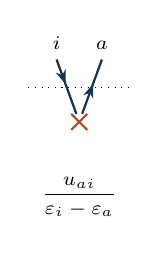
\begin{tikzpicture}[fcidiagram]
  \node[fvtx] (f) at (0,0.5) {};
  \draw[hline] (f) -- (-0.4,1.6); \draw[pline] (f) -- (0.4,1.6);
  \draw[dotted] (-0.9,1.1) -- (0.9,1.1);
  \node[dlab,above] at (-0.4,1.6) {$i$}; \node[dlab,above] at (0.4,1.6) {$a$};
  \node[dlab,below] at (0,-0.3) {$\dfrac{u_{ai}}{\varepsilon_i-\varepsilon_a}$};
\end{tikzpicture}
\hspace{3em}
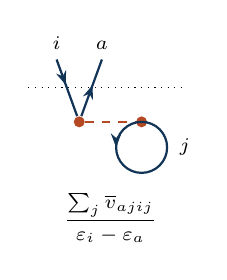
\begin{tikzpicture}[fcidiagram]
  \node[vtx] (v1) at (0,0.5) {}; \node[vtx] (v2) at (1.1,0.5) {}; \draw[vint] (v1) -- (v2);
  \draw[hline] (v1) -- (-0.4,1.6); \draw[pline] (v1) -- (0.4,1.6);
  \draw[hloop] (1.1,0.05) ++(0.45,0) arc (0:360:0.45);
  \draw[dotted] (-0.9,1.1) -- (1.9,1.1);
  \node[dlab,above] at (-0.4,1.6) {$i$}; \node[dlab,above] at (0.4,1.6) {$a$};
  \node[dlab,right] at (1.6,0.05) {$j$};
  \node[dlab,below] at (0.55,-0.6) {$\dfrac{\sum_j\vbar{a}{j}{i}{j}}{\varepsilon_i-\varepsilon_a}$};
\end{tikzpicture}
\hspace{3em}
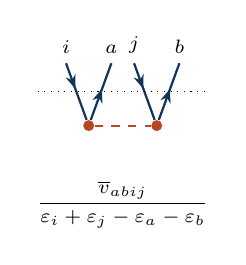
\begin{tikzpicture}[fcidiagram]
  \node[vtx] (v1) at (0,0.5) {}; \node[vtx] (v2) at (1.2,0.5) {}; \draw[vint] (v1) -- (v2);
  \draw[hline] (v1) -- (-0.4,1.6); \draw[pline] (v1) -- (0.4,1.6);
  \draw[hline] (v2) -- (0.8,1.6); \draw[pline] (v2) -- (1.6,1.6);
  \draw[dotted] (-0.9,1.1) -- (2.1,1.1);
  \node[dlab,above] at (-0.4,1.6) {$i$}; \node[dlab,above] at (0.4,1.6) {$a$};
  \node[dlab,above] at (0.8,1.6) {$j$}; \node[dlab,above] at (1.6,1.6) {$b$};
  \node[dlab,below] at (0.6,-0.3) {$\dfrac{\vbar{a}{b}{i}{j}}{\varepsilon_i+\varepsilon_j-\varepsilon_a-\varepsilon_b}$};
\end{tikzpicture}
\end{center}
\begin{itemize}
\item \alert{Open} diagrams: lines leave through the top. The cut above the vertex is crossed by the open lines and gives the denominator; an amplitude with $n$ vertices has $n$ cuts.
\item The first two are the Fock-matrix vertices, $u_{ai}+\sum_j\vbar{a}{j}{i}{j}=f_{ai}$ (Brillouin: zero in a HF basis); the third is the pair-creation vertex $B$ of the RPA. Chapter 5 drew these amplitudes as \emph{bars}; perturbation theory replaces the bar by the vertices that generate it.
\end{itemize}
\end{frame}

\begin{frame}{Second order, 1: connected open diagrams}
\small
$\Omega^{(2)}=RVRV-E^{(1)}R^2V$. Put a second vertex on top of a first-order piece and contract at least one line between them. Three of the many:
\begin{center}
\begin{tabular}{@{}c@{\hspace{3em}}c@{\hspace{3em}}c@{}}
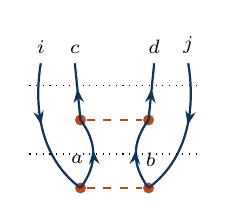
\begin{tikzpicture}[fcidiagram]
  \node[vtx] (b1) at (0,0) {}; \node[vtx] (b2) at (1.2,0) {}; \draw[vint] (b1) -- (b2);
  \node[vtx] (m1) at (0,1.2) {}; \node[vtx] (m2) at (1.2,1.2) {}; \draw[vint] (m1) -- (m2);
  \draw[pline] (b1.center) .. controls (0.3,0.4) and (0.3,0.8) .. (m1.center);
  \draw[pline] (b2.center) .. controls (0.9,0.4) and (0.9,0.8) .. (m2.center);
  \draw[pline] (m1.center) -- (-0.1,2.2); \draw[pline] (m2.center) -- (1.3,2.2);
  \draw[hline] (b1.center) .. controls (-0.8,0.6) and (-0.8,1.6) .. (-0.7,2.2);
  \draw[hline] (b2.center) .. controls (2.0,0.6) and (2.0,1.6) .. (1.9,2.2);
  \draw[dotted] (-0.9,0.6) -- (2.1,0.6); \draw[dotted] (-0.9,1.8) -- (2.1,1.8);
  \node[dlab,left] at (0.22,0.5) {$a$}; \node[dlab,right] at (0.98,0.5) {$b$};
  \node[dlab,above] at (-0.1,2.2) {$c$}; \node[dlab,above] at (1.3,2.2) {$d$};
  \node[dlab,above] at (-0.7,2.2) {$i$}; \node[dlab,above] at (1.9,2.2) {$j$};
\end{tikzpicture}
&
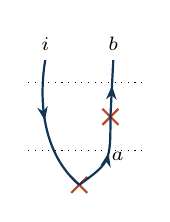
\begin{tikzpicture}[fcidiagram]
  \node[fvtx] (b) at (0,0) {}; \node[fvtx] (m) at (0.55,1.2) {};
  \draw[hline] (b.center) .. controls (-0.7,0.6) and (-0.7,1.6) .. (-0.6,2.2);
  \draw[pline] (b.center) .. controls (0.55,0.4) .. (m.center);
  \draw[pline] (m.center) -- (0.6,2.2);
  \draw[dotted] (-0.9,0.6) -- (1.1,0.6); \draw[dotted] (-0.9,1.8) -- (1.1,1.8);
  \node[dlab,right] at (0.4,0.5) {$a$}; \node[dlab,above] at (0.6,2.2) {$b$}; \node[dlab,above] at (-0.6,2.2) {$i$};
\end{tikzpicture}
&
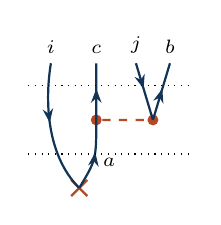
\begin{tikzpicture}[fcidiagram]
  \node[fvtx] (b) at (0,0) {};
  \node[vtx] (t1) at (0.3,1.2) {}; \node[vtx] (t2) at (1.3,1.2) {}; \draw[vint] (t1) -- (t2);
  \draw[hline] (b.center) .. controls (-0.6,0.6) and (-0.6,1.6) .. (-0.5,2.2);
  \draw[pline] (b.center) .. controls (0.3,0.5) .. (t1.center);
  \draw[pline] (t1.center) -- (0.3,2.2);
  \draw[hline] (t2.center) -- (1.0,2.2); \draw[pline] (t2.center) -- (1.6,2.2);
  \draw[dotted] (-0.9,0.6) -- (2.0,0.6); \draw[dotted] (-0.9,1.8) -- (2.0,1.8);
  \node[dlab,right] at (0.25,0.45) {$a$};
  \node[dlab,above] at (-0.5,2.2) {$i$}; \node[dlab,above] at (0.3,2.2) {$c$};
  \node[dlab,above] at (1.0,2.2) {$j$}; \node[dlab,above] at (1.6,2.2) {$b$};
\end{tikzpicture}
\\[0.4em]
pp ladder on a double & cross on the particle line & a double from a single and $V$
\end{tabular}
\end{center}
\[
\frac12\sum_{ab}\frac{\vbar{c}{d}{a}{b}\,\vbar{a}{b}{i}{j}}{\varepsilon_{ij}^{ab}\,\varepsilon_{ij}^{cd}},\qquad
\sum_a\frac{u_{ba}\,u_{ai}}{(\varepsilon_i-\varepsilon_a)(\varepsilon_i-\varepsilon_b)},\qquad\ldots
\]
\small These are \alert{connected}: a single piece. With a cut above the top vertex they are the amplitudes $\langle\Phi_{ij}^{cd}|\Psi^{(2)}\rangle$, $\langle\Phi_i^b|\Psi^{(2)}\rangle$, \dots\ -- the top vertex of a third-order \emph{energy} diagram would close them (below). The third picture: $\cre{a}$ of the single is contracted into the interaction, which creates $(b,j)$; its value has the ring/cross structure of diagram 3 of week 45, opened.
\end{frame}

\begin{frame}{Second order, 2: disconnected but linked}
\small
Two first-order pieces, \emph{no line between them}, both with open lines. Two time orderings, one drawing:
\begin{center}
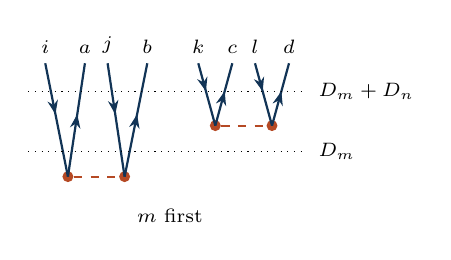
\begin{tikzpicture}[fcidiagram]
  \node[vtx] (a1) at (0,0) {}; \node[vtx] (a2) at (1.0,0) {}; \draw[vint] (a1) -- (a2);
  \draw[hline] (a1.center) -- (-0.4,2.0); \draw[pline] (a1.center) -- (0.3,2.0);
  \draw[hline] (a2.center) -- (0.7,2.0); \draw[pline] (a2.center) -- (1.4,2.0);
  \node[vtx] (b1) at (2.6,0.9) {}; \node[vtx] (b2) at (3.6,0.9) {}; \draw[vint] (b1) -- (b2);
  \draw[hline] (b1.center) -- (2.3,2.0); \draw[pline] (b1.center) -- (2.9,2.0);
  \draw[hline] (b2.center) -- (3.3,2.0); \draw[pline] (b2.center) -- (3.9,2.0);
  \draw[dotted] (-0.7,0.45) -- (4.2,0.45); \draw[dotted] (-0.7,1.5) -- (4.2,1.5);
  \node[dlab,right] at (4.25,0.45) {$D_m$}; \node[dlab,right] at (4.25,1.5) {$D_m+D_n$};
  \node[dlab,above] at (-0.4,2.0) {$i$}; \node[dlab,above] at (0.3,2.0) {$a$}; \node[dlab,above] at (0.7,2.0) {$j$}; \node[dlab,above] at (1.4,2.0) {$b$};
  \node[dlab,above] at (2.3,2.0) {$k$}; \node[dlab,above] at (2.9,2.0) {$c$}; \node[dlab,above] at (3.3,2.0) {$l$}; \node[dlab,above] at (3.9,2.0) {$d$};
  \node[dlab,below] at (1.8,-0.4) {$m$ first};
\end{tikzpicture}
\hspace{2em}
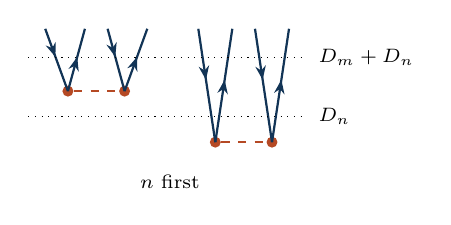
\begin{tikzpicture}[fcidiagram]
  \node[vtx] (a1) at (0,0.9) {}; \node[vtx] (a2) at (1.0,0.9) {}; \draw[vint] (a1) -- (a2);
  \draw[hline] (a1.center) -- (-0.4,2.0); \draw[pline] (a1.center) -- (0.3,2.0);
  \draw[hline] (a2.center) -- (0.7,2.0); \draw[pline] (a2.center) -- (1.4,2.0);
  \node[vtx] (b1) at (2.6,0) {}; \node[vtx] (b2) at (3.6,0) {}; \draw[vint] (b1) -- (b2);
  \draw[hline] (b1.center) -- (2.3,2.0); \draw[pline] (b1.center) -- (2.9,2.0);
  \draw[hline] (b2.center) -- (3.3,2.0); \draw[pline] (b2.center) -- (3.9,2.0);
  \draw[dotted] (-0.7,0.45) -- (4.2,0.45); \draw[dotted] (-0.7,1.5) -- (4.2,1.5);
  \node[dlab,right] at (4.25,0.45) {$D_n$}; \node[dlab,right] at (4.25,1.5) {$D_m+D_n$};
  \node[dlab,below] at (1.8,-0.4) {$n$ first};
\end{tikzpicture}
\end{center}
\[
\langle\Phi_{ijkl}^{abcd}|\Psi^{(2)}\rangle\ \ni\ \vbar{a}{b}{i}{j}\,\vbar{c}{d}{k}{l}\Bigl[\frac{1}{D_m(D_m+D_n)}+\frac{1}{D_n(D_m+D_n)}\Bigr]
=\frac{\vbar{a}{b}{i}{j}}{D_m}\cdot\frac{\vbar{c}{d}{k}{l}}{D_n}=t_m\,t_n
\]
\centerline{\small with $D_m=\varepsilon_{ij}^{ab}$, $D_n=\varepsilon_{kl}^{cd}$ and the same determinant phase in both orderings.}
\begin{itemize}
\item Disjoint orbitals: the energies add on the common cut, $D_{m\otimes n}=D_m+D_n$, and the two orderings sum to the \alert{product of the two first-order amplitudes}. The leading quadruple of $\Psi^{(2)}$ is a product of doubles (chapter 5: CID lacks it, that is why CID is not size consistent).
\item \alert{Disconnected but linked}: no piece is closed. Such terms belong to the wave function and are kept. (Friday: $e^{T}$ generates exactly these, as $\tfrac12T_2^2$.)
\end{itemize}
\end{frame}

\begin{frame}{Second order, 3: unlinked}
\small\tikzset{fcidiagram/.append style={scale=.60}}
Two pieces, no line between them, and \alert{one of them closed}: the first-order energy diagrams of week 45 (the $u$ loop, the two bubbles) floating next to an open first-order piece.
\begin{center}
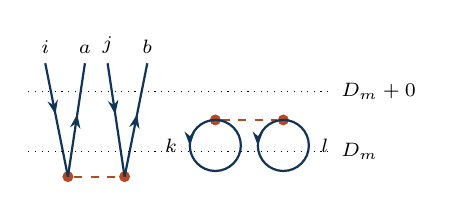
\begin{tikzpicture}[fcidiagram]
  \node[vtx] (a1) at (0,0) {}; \node[vtx] (a2) at (1.0,0) {}; \draw[vint] (a1) -- (a2);
  \draw[hline] (a1.center) -- (-0.4,2.0); \draw[pline] (a1.center) -- (0.3,2.0);
  \draw[hline] (a2.center) -- (0.7,2.0); \draw[pline] (a2.center) -- (1.4,2.0);
  \node[vtx] (b1) at (2.6,1.0) {}; \node[vtx] (b2) at (3.8,1.0) {}; \draw[vint] (b1) -- (b2);
  \draw[hloop] (2.6,0.55) ++(0.45,0) arc (0:360:0.45);
  \draw[hloop] (3.8,0.55) ++(0.45,0) arc (0:360:0.45);
  \node[dlab,left] at (2.1,0.55) {$k$}; \node[dlab,right] at (4.3,0.55) {$l$};
  \draw[dotted] (-0.7,0.45) -- (4.6,0.45); \draw[dotted] (-0.7,1.5) -- (4.6,1.5);
  \node[dlab,right] at (4.65,0.45) {$D_m$}; \node[dlab,right] at (4.65,1.5) {$D_m+0$};
  \node[dlab,above] at (-0.4,2.0) {$i$}; \node[dlab,above] at (0.3,2.0) {$a$}; \node[dlab,above] at (0.7,2.0) {$j$}; \node[dlab,above] at (1.4,2.0) {$b$};
\end{tikzpicture}
\hspace{2.5em}
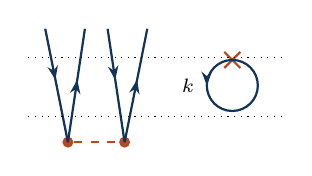
\begin{tikzpicture}[fcidiagram]
  \node[vtx] (a1) at (0,0) {}; \node[vtx] (a2) at (1.0,0) {}; \draw[vint] (a1) -- (a2);
  \draw[hline] (a1.center) -- (-0.4,2.0); \draw[pline] (a1.center) -- (0.3,2.0);
  \draw[hline] (a2.center) -- (0.7,2.0); \draw[pline] (a2.center) -- (1.4,2.0);
  \node[fvtx] (f) at (2.9,1.45) {};
  \draw[hloop] (2.9,1.0) ++(0.45,0) arc (0:360:0.45);
  \node[dlab,left] at (2.4,1.0) {$k$};
  \draw[dotted] (-0.7,0.45) -- (3.8,0.45); \draw[dotted] (-0.7,1.5) -- (3.8,1.5);
\end{tikzpicture}
\end{center}
\begin{columns}[T]
\column{0.55\textwidth}
\begin{block}{Read with the rules}
The closed piece adds no line to the second cut, so both denominators are $D_m$; its value is $\tfrac12\sum_{kl}\vbar{k}{l}{k}{l}$ or $\sum_k u_{kk}$, together $E^{(1)}=V_{00}$:
\[
\text{unlinked part of }\langle\Phi_m|RVRV|\ph\rangle=\frac{V_{00}\,V_{m0}}{D_m^2}.
\]
The closed piece cannot act \emph{first}: $R_0E^{(1)}\ket{\ph}=0$ ($Q$).
\end{block}
\column{0.45\textwidth}
\begin{block}{The renormalisation term}
\[
-E^{(1)}R^2V\ket{\ph}\ \to\ -\frac{V_{00}V_{m0}}{D_m^2}.
\]
\alert{Exactly the unlinked diagram, with a minus sign.} What is left of $\Omega^{(2)}$ is linked: $\Omega^{(2)}=[RVRV]_{\rm linked}$.
\end{block}
\end{columns}
\vspace{0em}
\small Definitions. \emph{Connected}: one piece. \emph{Linked}: no closed piece hangs loose (disconnected open pieces allowed). \emph{Unlinked}: contains a closed piece with no line to the rest. For a closed (energy) diagram linked $=$ connected.
\end{frame}

\begin{frame}{Pause to think \#1}
\thinkq{4}{\normalsize Third order of the wave operator with bare vertices:
\[
\Omega^{(3)}=RVRVRV-E^{(1)}\bigl[RVR^2V+R^2VRV\bigr]+\bigl(E^{(1)}\bigr)^2R^3V-E^{(2)}R^2V.
\]
\begin{enumerate}
\item Which unlinked drawings does $RVRVRV$ contain? (A closed piece can have one or two vertices. It may begin before the open component, but cannot close before that component starts.)
\item Match each renormalisation term with one family of unlinked drawings. Where does the factor $(E^{(1)})^2$ come from with the sign $+$, and why does the $-E^{(2)}$ term need \emph{two} time orderings?
\end{enumerate}}
\end{frame}

\begin{frame}{Answer to pause \#1}
\thinka{\footnotesize%
Let $m$ denote the first excitation in the open component (creation value $V_{m0}$). The unlinked contributions are:
\begin{enumerate}
\item \textbf{One closed one-vertex piece} $E^{(1)}$, either between the two open vertices or above both: denominators $D_m,D_m,D_{m'}$ or $D_m,D_{m'},D_{m'}$ -- exactly $E^{(1)}[R^2VRV+RVR^2V]$, removed by the two mixed terms.
\item \textbf{Two closed one-vertex pieces}: $(E^{(1)})^2V_{m0}/D_m^3$ in the principal term; but the mixed terms contain it \emph{twice} (each $V$ in $RVR^2V$ still carries its $E^{(1)}$ part), so $+1-2=-1$, and $+(E^{(1)})^2R^3V$ restores zero.
\item \textbf{One closed two-vertex piece} $n$ (a second-order energy diagram) beside the open piece: two orderings, $n$ opened after or before $m$,
\[
\frac{1}{D_m(D_m+D_n)D_m}+\frac{1}{D_n(D_m+D_n)D_m}=\frac{1}{D_m^2D_n}
\quad\Longrightarrow\quad E^{(2)}\frac{V_{m0}}{D_m^2}:
\]
\alert{the factorisation of denominators}, and $-E^{(2)}R^2V$ removes it. (The ordering with $n$ opened and closed before $m$ starts is killed by $Q$.)
\end{enumerate}
Together the renormalisation terms cancel the unlinked sum, including the positive inclusion--exclusion correction: $\Omega^{(3)}=[RVRVRV]_{\rm linked}$.}
\end{frame}

\begin{frame}{From the wave operator to the energy: close with a vertex}
\small\tikzset{fcidiagram/.append style={scale=.60}}
$E^{(n+1)}=\av{V\Omega^{(n)}}$: put one more vertex on top and contract \emph{all} open lines into it.
\begin{center}
\begin{tabular}{@{}c@{\hspace{2.5em}}c@{\hspace{2.5em}}c@{}}
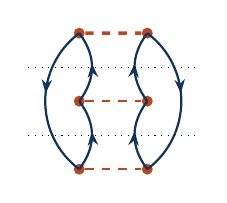
\begin{tikzpicture}[fcidiagram]
  \node[vtx] (b1) at (0,0) {}; \node[vtx] (b2) at (1.2,0) {}; \draw[vint] (b1) -- (b2);
  \node[vtx] (m1) at (0,1.2) {}; \node[vtx] (m2) at (1.2,1.2) {}; \draw[vint] (m1) -- (m2);
  \node[vtx] (t1) at (0,2.4) {}; \node[vtx] (t2) at (1.2,2.4) {}; \draw[vint,warm,very thick] (t1) -- (t2);
  \draw[pline] (b1.center) .. controls (0.3,0.4) and (0.3,0.8) .. (m1.center);
  \draw[pline] (b2.center) .. controls (0.9,0.4) and (0.9,0.8) .. (m2.center);
  \draw[pline] (m1.center) .. controls (0.3,1.6) and (0.3,2.0) .. (t1.center);
  \draw[pline] (m2.center) .. controls (0.9,1.6) and (0.9,2.0) .. (t2.center);
  \draw[hline] (b1.center) .. controls (-0.8,0.6) and (-0.8,1.8) .. (t1.center);
  \draw[hline] (b2.center) .. controls (2.0,0.6) and (2.0,1.8) .. (t2.center);
  \draw[dotted] (-0.9,0.6) -- (2.1,0.6); \draw[dotted] (-0.9,1.8) -- (2.1,1.8);
\end{tikzpicture}
&
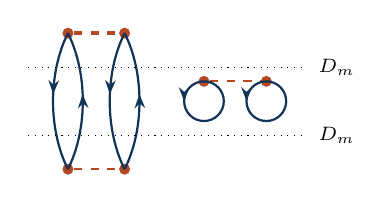
\begin{tikzpicture}[fcidiagram]
  \node[vtx] (a1) at (0,0) {}; \node[vtx] (a2) at (1.0,0) {}; \draw[vint] (a1) -- (a2);
  \node[vtx] (t1) at (0,2.4) {}; \node[vtx] (t2) at (1.0,2.4) {}; \draw[vint,warm,very thick] (t1) -- (t2);
  \draw[pline] (a1.center) .. controls (0.35,0.7) and (0.35,1.7) .. (t1.center);
  \draw[hline] (a1.center) .. controls (-0.35,0.7) and (-0.35,1.7) .. (t1.center);
  \draw[pline] (a2.center) .. controls (1.35,0.7) and (1.35,1.7) .. (t2.center);
  \draw[hline] (a2.center) .. controls (0.65,0.7) and (0.65,1.7) .. (t2.center);
  \node[vtx] (b1) at (2.4,1.55) {}; \node[vtx] (b2) at (3.5,1.55) {}; \draw[vint] (b1) -- (b2);
  \draw[hloop] (2.4,1.2) ++(0.35,0) arc (0:360:0.35);
  \draw[hloop] (3.5,1.2) ++(0.35,0) arc (0:360:0.35);
  \draw[dotted] (-0.7,0.6) -- (4.2,0.6); \draw[dotted] (-0.7,1.8) -- (4.2,1.8);
  \node[dlab,right] at (4.25,0.6) {$D_m$}; \node[dlab,right] at (4.25,1.8) {$D_m$};
\end{tikzpicture}
&
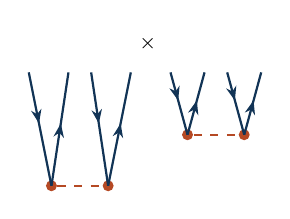
\begin{tikzpicture}[fcidiagram]
  \node[vtx] (a1) at (0,0) {}; \node[vtx] (a2) at (1.0,0) {}; \draw[vint] (a1) -- (a2);
  \draw[hline] (a1.center) -- (-0.4,2.0); \draw[pline] (a1.center) -- (0.3,2.0);
  \draw[hline] (a2.center) -- (0.7,2.0); \draw[pline] (a2.center) -- (1.4,2.0);
  \node[vtx] (b1) at (2.4,0.9) {}; \node[vtx] (b2) at (3.4,0.9) {}; \draw[vint] (b1) -- (b2);
  \draw[hline] (b1.center) -- (2.1,2.0); \draw[pline] (b1.center) -- (2.7,2.0);
  \draw[hline] (b2.center) -- (3.1,2.0); \draw[pline] (b2.center) -- (3.7,2.0);
  \node[dlab] at (1.7,2.5) {\alert{$\times$}};
\end{tikzpicture}
\\[0.3em]
connected $\to$ connected closed & unlinked $\to$ \alert{unlinked closed} & \parbox{3.6cm}{\centering disconnected-but-linked $\to$ nothing:\\ one vertex cannot close eight lines}
\end{tabular}
\end{center}
\begin{itemize}
\item Middle: the third-order \emph{energy} diagram with a closed first-order piece between the cuts, $E^{(1)}\sum_m|V_{m0}|^2/D_m^2=E^{(1)}\av{VR^2V}$ -- the renormalisation term of $E^{(3)}$ with the opposite sign. Pairing model, $g=0.5$: $E^{(1)}=-g=-0.5$, $\av{VR^2V}=\tfrac{29}{288}g^2=0.0251736$, unlinked diagram $-0.0125868$, cancelled by the folded contribution $+0.0125868$.
\item Right: a quadruple cannot be closed by one interaction, so it contributes to $E^{(3)}$ nothing; a further vertex can bring it back to a double, and then it is the connected fourth-order diagram with two pairs created, scattered into each other, closed.
\item \alert{The sum of the renormalisation terms cancels the unlinked energy contributions}, order by order. At higher orders this includes positive inclusion--exclusion terms.
\end{itemize}
\end{frame}

\begin{frame}{Disconnected open pieces can give a connected energy diagram}
\small
The number of external lines matters. A two-body interaction can close two singles, but cannot close two doubles at once.
\[
 T_1^{(1)}=\sum_{ia}\frac{\ftil{ai}}{\varepsilon_i-\varepsilon_a}\cre{a}\ann{i},
 \qquad \ket{\Psi^{(2)}}\supset\tfrac12(T_1^{(1)})^2\ket{\ph}.
\]
The two singles have no contraction between them. Closing all four external lines with one two-body interaction connects the whole energy graph:
\[
 E^{(3)}\supset\frac12\sum_{ijab}\vbar{i}{j}{a}{b}
 \frac{\ftil{ai}}{\varepsilon_i-\varepsilon_a}
 \frac{\ftil{bj}}{\varepsilon_j-\varepsilon_b}.
\]
The $1/2$ comes from the exponential and the complete antisymmetric contraction. The two relative time orderings give the product of denominators.
\begin{block}{Scope of the preceding picture}
The eight external lines of two doubles cannot be closed by one two-body vertex. Disconnected but linked open diagrams are not generally excluded from the energy; they contribute whenever the closing vertex can join all their components.
\end{block}
\end{frame}


\begin{frame}{Pause to think \#2}
\thinkq{3}{Pairing model with bare vertices ($u=0$, so $E^{(1)}=\tfrac12\sum_{ij}\vbar{i}{j}{i}{j}=-g$ for two pairs).
\begin{enumerate}
\item Draw the unlinked third-order energy diagrams: which closed one-vertex pieces exist, and between which cuts can they sit?
\item Last week the \emph{connected} third order was ``ladders $-0.0230035$ $+$ hole insertion $+0.0125868$'' with normal-ordered vertices. With bare vertices the hole insertion $\ftil{ii}=U_{ii}=-g/2$ is a bubble on a hole line. Where did the $+0.0125868$ come from, and where does the unlinked $-0.0125868$ go?
\end{enumerate}}
\end{frame}

\begin{frame}{Answer to pause \#2}
\thinka{\footnotesize%
\begin{enumerate}
\item One closed piece: the two bubbles joined by an interaction, $\tfrac12\sum_{kl}\vbar{k}{l}{k}{l}=-g$ (there is no $u$ loop). It sits between the two cuts of a second-order ring, the only second-order diagram of the pairing model: one unlinked diagram per double $m$, worth $-g\,|V_{m0}|^2/D_m^2$, in total $-0.0125868$.
\item With bare vertices the principal term $\av{VRVRV}=-0.0230035$ is the sum of \emph{four} families: pp ladder $-0.0115017$, hh ladder $-0.0115017$, bubbles on the two hole lines $+0.0125868$, and the unlinked diagram $-0.0125868$. For the pairing model the last two cancel each other exactly ($W_{mm}=V_{mm}-V_{00}=0$: the diagonal ladder elements $-g/2-g/2$ are undone by the two hole bubbles $+g/2+g/2$), which is why the principal term \emph{looks} like the ladders alone. The renormalisation term $-E^{(1)}\av{VR^2V}=+0.0125868$ removes the unlinked diagram, and what survives is connected: ladders $+$ hole bubbles $=-0.0104167=E^{(3)}$. Normal ordering does the same bookkeeping in one step: the bubble becomes the cross $\ftil{ii}=-g/2$ and the unlinked diagram never appears.
\end{enumerate}}
\end{frame}
\begin{frame}{Normal ordering removes the one-vertex closed pieces}
\small
\small
Every closed piece with \emph{one} vertex is a reference expectation value, $\av{H_I}=E^{(1)}$. Writing $H_I=E^{(1)}+W$ with $W$ normal ordered (week 45, step zero):
\begin{align*}
\av{W}&=0,\qquad
\Omega^{(2)}=RWRW,\qquad \Omega^{(3)}=RWRWRW-E^{(2)}R^2W,\\
E^{(3)}&=\av{WRWRW},\qquad E^{(4)}=\av{WRWRWRW}-E^{(2)}\av{WR^2W}.
\end{align*}
\begin{itemize}
\item A normal-ordered vertex has no contraction with itself: no bubbles, no $u$ loop, hence no closed one-vertex piece. The unlinked drawings of pause \#1 with $E^{(1)}$ pieces are gone, and so are the renormalisation terms that cancelled them.
\item The smallest closed piece is now a \emph{second-order} energy diagram (ring, or two crosses), and the first place it can float beside something is $\Omega^{(3)}$ (pause \#1, item 3) and, for the energy, $E^{(4)}$.
\item From here on all vertices are normal ordered: a cross is $\ftil{pq}=f_{pq}-\varepsilon_p\delta_{pq}$, an interaction is $\vbar{p}{q}{r}{s}$.
\end{itemize}
Pairing, $g=0.5$: $\av{WR_0WR_0W}=-0.01041667$. At fourth order the folded term is still needed for additivity of independent copies.
\end{frame}

\begin{frame}{Fourth order: a new kind of drawing}
\[
E^{(4)}=\av{WR_0WR_0WR_0W}-E^{(2)}\av{WR_0^2W}.
\]
With four normal-ordered vertices a complete contraction can fall into \alert{two closed pieces of two vertices each}:
\begin{center}
\begin{tabular}{lll}
\toprule
pairing of vertices & intermediate states & \\
\midrule
\(1\)--\(3\) and \(2\)--\(4\) & \(m,\ m\otimes n,\ n\) & unlinked, overlapping in time\\
\(1\)--\(4\) and \(2\)--\(3\) & \(m,\ m\otimes n,\ m\) & unlinked, overlapping in time\\
\(1\)--\(2\) and \(3\)--\(4\) & \(m,\ \ph,\ n\) & \alert{zero}: no line crosses the middle cut, \(Q\) kills it\\
\bottomrule
\end{tabular}
\end{center}
\begin{itemize}
\item Each piece is a closed second-order diagram -- a ring, or two crosses.
\item Such a drawing is \alert{unlinked}: it contains a closed part with no line connecting it to the rest.
\item With four normal-ordered vertices the remaining nonzero closed topologies are connected. The unlinked sum is $+E^{(2)}\av{WR_0^2W}$; the folded contribution is its negative.
\end{itemize}
\end{frame}

\begin{frame}{The two unlinked time orderings, drawn}
\begin{center}
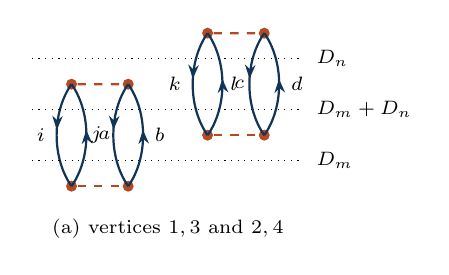
\begin{tikzpicture}[fcidiagram]
  % piece A: vertices 1 (y=0) and 3 (y=1.8); piece B: vertices 2 (y=0.9) and 4 (y=2.7)
  \node[vtx] (a1) at (0,0) {}; \node[vtx] (a2) at (1.0,0) {}; \draw[vint] (a1) -- (a2);
  \node[vtx] (a3) at (0,1.8) {}; \node[vtx] (a4) at (1.0,1.8) {}; \draw[vint] (a3) -- (a4);
  \draw[pline] (a1.center) .. controls (0.35,0.5) and (0.35,1.3) .. (a3.center);
  \draw[hline] (a1.center) .. controls (-0.35,0.5) and (-0.35,1.3) .. (a3.center);
  \draw[pline] (a2.center) .. controls (1.35,0.5) and (1.35,1.3) .. (a4.center);
  \draw[hline] (a2.center) .. controls (0.65,0.5) and (0.65,1.3) .. (a4.center);
  \node[vtx] (b1) at (2.4,0.9) {}; \node[vtx] (b2) at (3.4,0.9) {}; \draw[vint] (b1) -- (b2);
  \node[vtx] (b3) at (2.4,2.7) {}; \node[vtx] (b4) at (3.4,2.7) {}; \draw[vint] (b3) -- (b4);
  \draw[pline] (b1.center) .. controls (2.75,1.4) and (2.75,2.2) .. (b3.center);
  \draw[hline] (b1.center) .. controls (2.05,1.4) and (2.05,2.2) .. (b3.center);
  \draw[pline] (b2.center) .. controls (3.75,1.4) and (3.75,2.2) .. (b4.center);
  \draw[hline] (b2.center) .. controls (3.05,1.4) and (3.05,2.2) .. (b4.center);
  \draw[dotted] (-0.7,0.45) -- (4.1,0.45); \draw[dotted] (-0.7,1.35) -- (4.1,1.35); \draw[dotted] (-0.7,2.25) -- (4.1,2.25);
  \node[dlab,right] at (4.15,0.45) {$D_m$}; \node[dlab,right] at (4.15,1.35) {$D_m+D_n$}; \node[dlab,right] at (4.15,2.25) {$D_n$};
  \node[dlab,left] at (-0.3,0.9) {$i$}; \node[dlab,right] at (0.3,0.9) {$a$};
  \node[dlab,left] at (0.7,0.9) {$j$}; \node[dlab,right] at (1.3,0.9) {$b$};
  \node[dlab,left] at (2.1,1.8) {$k$}; \node[dlab,right] at (2.7,1.8) {$c$};
  \node[dlab,left] at (3.1,1.8) {$l$}; \node[dlab,right] at (3.7,1.8) {$d$};
  \node[dlab,below] at (1.7,-0.4) {(a) vertices $1,3$ and $2,4$};
\end{tikzpicture}
\hspace{2.5em}
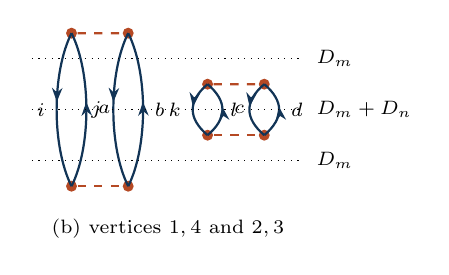
\begin{tikzpicture}[fcidiagram]
  % piece A: vertices 1 (y=0) and 4 (y=2.7); piece B: vertices 2 (y=0.9) and 3 (y=1.8)
  \node[vtx] (a1) at (0,0) {}; \node[vtx] (a2) at (1.0,0) {}; \draw[vint] (a1) -- (a2);
  \node[vtx] (a3) at (0,2.7) {}; \node[vtx] (a4) at (1.0,2.7) {}; \draw[vint] (a3) -- (a4);
  \draw[pline] (a1.center) .. controls (0.35,0.7) and (0.35,2.0) .. (a3.center);
  \draw[hline] (a1.center) .. controls (-0.35,0.7) and (-0.35,2.0) .. (a3.center);
  \draw[pline] (a2.center) .. controls (1.35,0.7) and (1.35,2.0) .. (a4.center);
  \draw[hline] (a2.center) .. controls (0.65,0.7) and (0.65,2.0) .. (a4.center);
  \node[vtx] (b1) at (2.4,0.9) {}; \node[vtx] (b2) at (3.4,0.9) {}; \draw[vint] (b1) -- (b2);
  \node[vtx] (b3) at (2.4,1.8) {}; \node[vtx] (b4) at (3.4,1.8) {}; \draw[vint] (b3) -- (b4);
  \draw[pline] (b1.center) .. controls (2.75,1.2) and (2.75,1.5) .. (b3.center);
  \draw[hline] (b1.center) .. controls (2.05,1.2) and (2.05,1.5) .. (b3.center);
  \draw[pline] (b2.center) .. controls (3.75,1.2) and (3.75,1.5) .. (b4.center);
  \draw[hline] (b2.center) .. controls (3.05,1.2) and (3.05,1.5) .. (b4.center);
  \draw[dotted] (-0.7,0.45) -- (4.1,0.45); \draw[dotted] (-0.7,1.35) -- (4.1,1.35); \draw[dotted] (-0.7,2.25) -- (4.1,2.25);
  \node[dlab,right] at (4.15,0.45) {$D_m$}; \node[dlab,right] at (4.15,1.35) {$D_m+D_n$}; \node[dlab,right] at (4.15,2.25) {$D_m$};
  \node[dlab,left] at (-0.3,1.35) {$i$}; \node[dlab,right] at (0.3,1.35) {$a$};
  \node[dlab,left] at (0.7,1.35) {$j$}; \node[dlab,right] at (1.3,1.35) {$b$};
  \node[dlab,left] at (2.1,1.35) {$k$}; \node[dlab,right] at (2.7,1.35) {$c$};
  \node[dlab,left] at (3.1,1.35) {$l$}; \node[dlab,right] at (3.7,1.35) {$d$};
  \node[dlab,below] at (1.7,-0.4) {(b) vertices $1,4$ and $2,3$};
\end{tikzpicture}
\end{center}
\small Two second-order rings, pairs \((ab,ij)\) and \((cd,kl)\) sharing no orbital; \(D_m=\varepsilon_{ij}^{ab}\), \(D_n=\varepsilon_{kl}^{cd}\) are the denominators of the rings on their own. The matrix elements, the weights and the signs of the two pieces simply \emph{multiply} (the line and loop counts add in the exponent). Only the denominators are not local to a piece: in the middle both rings are open, and the energies \emph{add} because the excitations involve different orbitals.
\end{frame}

\begin{frame}{The factorisation of the denominators}
Ordering (a): cuts \(D_m\), \(D_m+D_n\), \(D_n\). Ordering (b): \(D_m\), \(D_m+D_n\), \(D_m\). Add them:
\[
\boxed{\frac{1}{D_m(D_m+D_n)D_n}+\frac{1}{D_m(D_m+D_n)D_m}
=\frac{1}{D_m(D_m+D_n)}\cdot\frac{D_m+D_n}{D_mD_n}
=\frac{1}{D_m^2\,D_n}.}
\]
For fixed $m$ opened first, the two orders sum to $1/(D_m^2D_n)$. When $n$ opens first they give $1/(D_n^2D_m)$. An ordered double sum already includes the interchange of $m$ and $n$.
\begin{block}{Compare with the folded term}
\[
E^{(2)}\av{WR_0^2W}=\sum_{m,n\ne0}\frac{W_{0n}W_{n0}}{D_n}\,\frac{W_{0m}W_{m0}}{D_m^2}
\]
This product enters $E^{(4)}$ with a minus sign. For disjoint excitations it cancels the sum of the two overlapping orderings for each ordered pair of excitations.
\end{block}
For shared orbital labels, independent sums also contain formal EPV pairings. We will track their exchange partners explicitly after the proof.
\end{frame}

% ======================================================================
\section[Thursday 2: The proof]{Thursday, lecture 2: The theorem and its proof}
% ======================================================================

\begin{frame}{Factorisation for two open excitation histories}
Fix the vertex order \emph{within} each of two independent pieces. Let $A_r$ and $B_s$ be their signed energy deficits after $r$ and $s$ vertices. Put $A_0=B_0=0$. Let $S_{rs}$ sum the denominator products of all interleavings of these prefixes, including their final cut.
\[
 S_{r0}=\prod_{u=1}^r A_u^{-1},\quad S_{0s}=\prod_{v=1}^s B_v^{-1},\quad S_{00}=1.
\]
The last vertex belongs to one of the pieces. Their deficits add on the common cut, so for $r,s>0$,
\[
 S_{rs}=\frac{S_{r-1,s}+S_{r,s-1}}{A_r+B_s}
 =\frac{A_r+B_s}{A_r+B_s}
   \prod_{u=1}^r\frac1{A_u}\prod_{v=1}^s\frac1{B_v}.
\]
The second equality uses the induction hypothesis. This proves factorisation for prefixes with nonzero denominators. At a closed energy graph's final vertex there is no final denominator. The preceding fourth-order example treated that endpoint explicitly.
\end{frame}

\begin{frame}{Factorisation when one component closes}
\small
Let $A_1,\ldots,A_p$ be the nonzero deficits of an open history and let $B_1,\ldots,B_{q-1}\ne0$, $B_q=0$ describe a closed history.
\begin{block}{The boundary condition comes from $Q$}
The closed history cannot finish before the open history starts: set $S_{0q}=0$. Do not substitute $B_q=0$ into the open-history product, which would divide by zero.
\end{block}
For $r\ge1$, the same last-vertex recursion gives
\[
 S_{rq}=\frac{S_{r-1,q}+S_{r,q-1}}{A_r},\qquad
 S_{r,q-1}=\prod_{u=1}^r A_u^{-1}\prod_{v=1}^{q-1}B_v^{-1}.
\]
Induction from $S_{0q}=0$ yields
\[
 \boxed{S_{pq}=\left(\prod_{u=1}^{p}\frac1{A_u}\right)
 \left(\prod_{v=1}^{q-1}\frac1{B_v}\right)
 \sum_{j=1}^{p}\frac1{A_j}.}
\]
The last sum places an additional resolvent on each interval of the open history in turn. These are the squared denominators in the folded terms.
\end{frame}

\begin{frame}{A closed component: the five allowed interleavings}
Take an open history $A_1,A_2$ with deficits $a,b$ and a closed history $B_1,B_2$ with deficits $c,0$. Each row includes the final cut of the open amplitude.
\begin{center}
\setlength{\tabcolsep}{12pt}\begin{tabular}{lll}
\toprule
Order & cut deficits & denominator product\\
\midrule
$A_1A_2B_1B_2$ & $a,b,b+c,b$ & $[ab^2(b+c)]^{-1}$\\
$A_1B_1A_2B_2$ & $a,a+c,b+c,b$ & $[a(a+c)(b+c)b]^{-1}$\\
$A_1B_1B_2A_2$ & $a,a+c,a,b$ & $[a^2(a+c)b]^{-1}$\\
$B_1A_1A_2B_2$ & $c,a+c,b+c,b$ & $[c(a+c)(b+c)b]^{-1}$\\
$B_1A_1B_2A_2$ & $c,a+c,a,b$ & $[c(a+c)ab]^{-1}$\\
\bottomrule
\end{tabular}
\end{center}
The sixth ordering, $B_1B_2A_1A_2$, has an empty cut and is killed by $Q$. The five surviving terms sum to
\[
 \frac1{abc}\left(\frac1a+\frac1b\right).
\]
The closed two-vertex component supplies $E^{(2)}$; the two terms place $R_0^2$ on either open interval. Closing the open history gives fifth-order energy contributions.
\end{frame}


\begin{frame}{The linked-diagram theorem for a single reference}
\small
Assume a finite orbital basis and a nondegenerate, gapped ground determinant $\ket{\ph}$ of $H_0$. Follow its ground-state branch for small coupling $\lambda$. As before,
$H(\lambda)=H_0+\lambda(E^{(1)}+W)$ with $\av{W}=0$.
\begin{block}{Energy}
For $n\ge2$, sum the connected closed Wick diagrams with unrestricted line labels and the cut denominators of the indicated string.
\[
 E^{(n)}=\big[\av{W(R_0W)^{n-1}}\big]_{\rm connected},
 \qquad E_0(\lambda)=\varepsilon_0+\lambda E^{(1)}+\sum_{n\ge2}\lambda^n E^{(n)} .
\]
\end{block}
\begin{block}{Wave operator}
With $\braket{\ph}{\Psi_0(\lambda)}=1$, each component of a diagram for an excited-determinant amplitude must reach an external line. Several components may survive if each reaches the projecting bra. The diagram restriction is made in the Wick expansion, before imposing any separate determinant-state interpretation on a cut.
\end{block}
\end{frame}

\begin{frame}{Proof 1. Projection onto the interacting ground state}
Remove the scalar shift by writing $H'=H_0+\lambda W$. Define
\[
 U_T=e^{-T(H'-\varepsilon_0)},\qquad
 Z(T)=\av{U_T}=\sum_\nu |\braket{\Psi'_\nu}{\ph}|^2 e^{-T(E'_\nu-\varepsilon_0)}.
\]
Here the spectral eigenvectors are unit normalised. The ground-state overlap is nonzero for sufficiently small $\lambda$. The gap suppresses the excited terms, giving
\[
 E'_0-\varepsilon_0=-\lim_{T\to\infty}\partial_T\log Z(T),\qquad
 \ket{\Psi_0(\lambda)}=\lim_{T\to\infty}\frac{U_T\ket{\ph}}{Z(T)} .
\]
The ratio has reference overlap one at every $T$. Since
$\bra{\ph}(H_0-\varepsilon_0)=0$, the energy also has a form with one marked, latest vertex:
\[
 -\partial_T\log Z(T)=\lambda\frac{\av{W U_T}}{Z(T)} .
\]
\end{frame}

\begin{frame}{Proof 2. Independent vacuum components factorise}
Let $W_I(t)=e^{tH_0}W e^{-tH_0}$ and let $\mathcal T$ put later times on the left. The Dyson series on the reference gives
\[
 Z(T)=\sum_{N\ge0}\frac{(-\lambda)^N}{N!}
 \int_{[-T,0]^N}\!\dd^Nt\,
 \av{\mathcal T W_I(t_1)\cdots W_I(t_N)} .
\]
Wick contractions partition the $N$ labelled vertices into connected components. If there is no line between two sets, their orbital labels are summed independently and their time variables are integrated over a product domain. The signed integrand factorises because every closed component has even fermion parity.
\begin{block}{Relative time orderings}
For two components the Cartesian product of their ordered time domains splits into all interleavings that preserve each internal ordering. One ordering on its own need not factorise. Integrating over their union gives the product of the two component integrals.
\end{block}
\end{frame}

\begin{frame}{Proof 3. Counting the components produces an exponential}
Group connected vacuum graphs by type $\alpha$. Write $C_\alpha(T)$ for the signed, integrated weight of one component, with its vertex factorial and internal symmetry factors. Suppose $m_\alpha$ components of type $\alpha$ occur, each with $r_\alpha$ vertices, so $N=\sum_\alpha m_\alpha r_\alpha$. The number of partitions of the vertex labels is
\[
 \frac{N!}{\prod_\alpha (r_\alpha!)^{m_\alpha}m_\alpha!}.
\]
The Dyson $1/N!$ cancels the numerator. Each $1/r_\alpha!$ belongs to one component. Permuting identical components leaves the factor $1/m_\alpha!$. Summing their multiplicities gives
\[
 Z(T)=\prod_\alpha\sum_{m\ge0}\frac{C_\alpha(T)^m}{m!}
     =\exp\Bigl[\sum_\alpha C_\alpha(T)\Bigr].
\]
For example, $\av{W}=0$ implies $Z_1=0$. If $Z=1+\sum_n\lambda^n Z_n$, the fourth-order coefficient of $\log Z$ is $Z_4-Z_2^2/2$. The identical pair of second-order vacuum components cancels exactly.
\end{frame}

\begin{frame}{Proof 4. The energy selects one connected component}
In $\av{W U_T}$, distinguish the vertex $W$ at time zero. Every fully contracted term has a unique component containing this vertex. All other components are ordinary vacuum components. For $N$ integrated vertices, choosing the $k$ that join the marked component gives
\[
 \frac{1}{N!}\binom Nk=\frac{1}{k!(N-k)!}.
\]
The unmarked vertices therefore generate exactly $Z(T)$. If $M(T)$ sums the components attached to the marked vertex, then
\[
 \av{W U_T}=M(T) Z(T),\qquad E'_0-\varepsilon_0=\lambda\lim_{T\to\infty}M(T).
\]
Every interaction in $M$ is joined to the marked vertex by a path of fermion lines and interactions. Closing the external state with the reference gives a connected vacuum diagram. Equivalently, $-\partial_T\log Z$ selects the same connected series.
\end{frame}

\begin{frame}{Proof 5. Imaginary-time intervals give the Goldstone denominators}
Order the $n-1$ integrated vertices beneath the marked vertex $t_n=0$. During $s_k=t_{k+1}-t_k$ the free propagation supplies $e^{-\Delta_k s_k}$, with
\[
 \Delta_k=\sum_{a\ {\rm crossing}}\varepsilon_a-
           \sum_{i\ {\rm crossing}}\varepsilon_i=-D_k>0.
\]
Every cut of a connected closed graph crosses a line. At finite $T$, $s_k\ge0$ and $\sum_k s_k\le T$. As $T\to\infty$ the ordered integral, including its Dyson signs, becomes
\[
 (-1)^{n-1}\int_{[0,\infty)^{n-1}}\prod_{k=1}^{n-1}e^{-\Delta_k s_k}\dd s_k
 =\prod_{k=1}^{n-1}\frac{-1}{\Delta_k}=\prod_{k=1}^{n-1}\frac1{D_k}.
\]
Thus each connected, time-ordered graph has exactly the denominators, Wick sign and weight derived in week 45. Adding $\lambda E^{(1)}$ restores the energy of $H(\lambda)$. The small-coupling ground-state expansion is unique, so these are the RS energy coefficients.
\end{frame}

\begin{frame}{Why the long-time limit can be taken order by order}
In a finite basis, an isolated eigenvalue and its spectral projector are analytic near $\lambda=0$. Choose a small neighbourhood where the gap remains open and the reference overlap is nonzero. The spectral decomposition then has the form
\[
 Z(T,\lambda)=A(\lambda)e^{-T\delta E(\lambda)}[1+r_T(\lambda)],
 \quad A=|\braket{\Psi'_0}{\ph}|^2>0,
 \quad\delta E=E'_0-\varepsilon_0.
\]
For real $\lambda$ in this neighbourhood, excited-state terms decay exponentially. At every fixed derivative order $k$, their derivatives are bounded by a polynomial in $T$ times $e^{-\gamma T}$, for some $\gamma>0$. Therefore
\[
 \lim_{T\to\infty}\left.\partial_\lambda^k[-\partial_T\log Z(T,\lambda)]\right|_0
 =\left.\partial_\lambda^k\delta E(\lambda)\right|_0.
\]
At any fixed diagram order there are finitely many contractions and each connected time integral is convergent because every cut has a positive free excitation energy.
\begin{block}{What has been proved}
The connected diagrams give the RS Taylor coefficients. This does not prove convergence at physical coupling $\lambda=1$, at a level crossing, or in a gapless thermodynamic limit.
\end{block}
\end{frame}


\begin{frame}{Proof 6. Vacuum components cancel in the wave operator}
Project onto an excited determinant and divide by the vacuum amplitude:
\[
 c_\mu(\lambda)=\lim_{T\to\infty}\frac{\mel{\Phi_\mu}{U_T}{\ph}}{Z(T)}.
\]
Represent the bra by its external annihilators and creators at time zero. In every numerator graph, separate the components that reach at least one external line from those that reach none. Choosing the vertices in the second set produces the same binomial factor as in the energy proof. Their sum is $Z(T)$ and cancels at finite $T$.
\[
 \ket{\Psi_0(\lambda)}=\ket{\ph}
   +\sum_{n\ge1}\lambda^n\big[(R_0 W)^n\ket{\ph}\big]_{\rm linked}.
\]
Here brackets instruct us to retain the indicated Wick diagrams with their line denominators. The open graph has one more interval, between its last interaction and its external bra. This supplies the leftmost $R_0$. Distinct open components may end on different external legs.
\end{frame}

\begin{frame}{A disconnected contribution to a linked amplitude}
Let $m$ and $n$ be independent double excitations on disjoint orbitals with deficits $D_m$ and $D_n$. Project onto their combined quadruple excitation and fix the same determinant phase in both time orderings. Even excitation operators on disjoint orbitals commute. The two terms have denominators
\[
 \frac{1}{D_m(D_m+D_n)}+\frac{1}{D_n(D_m+D_n)}
 =\frac{1}{D_mD_n}.
\]
Multiplying by the two creation matrix elements gives the product of the first-order doubles amplitudes (with the chosen determinant phase). Each component reaches the quadruple bra. A detached vacuum bubble would instead multiply the numerator by a factor already present in $Z(T)$.
\medskip

\footnotesize Further reading: J. Goldstone, \href{https://doi.org/10.1098/rspa.1957.0037}{Proc. R. Soc. A \textbf{239} (1957)}. I. Shavitt and R. J. Bartlett, \emph{Many-Body Methods in Chemistry and Physics}, \S5.7.5 (EPV terms) and \href{https://doi.org/10.1017/CBO9780511596834.007}{chapter 6} (linked diagrams).
\end{frame}

\begin{frame}{Pauli exclusion at an intermediate cut}
Consider two overlapping single excitations $X=\cre{a}\ann{i}$ and $Y=\cre{b}\ann{i}$, with $a\ne b$. Each excitation is allowed on its own. Together they would empty the same occupied spin orbital twice:
\[
 YX\ket{\ph}=\cre{b}\ann{i}\cre{a}\ann{i}\ket{\ph}
 =-\cre{b}\cre{a}\ann{i}^{\,2}\ket{\ph}=0 .
\]
Creating two particles in the same virtual spin orbital also gives zero, since $(\cre{a})^2=0$. Reusing a label \emph{after} its line has ended can describe a legitimate excitation.
\begin{block}{Where an exclusion-principle-violating (EPV) term enters}
A determinant sum contains only admissible intermediate states. An individual Wick pairing sums the orbital labels of its lines independently. Two distinct lines present at the same cut can then acquire the same hole or particle label. The cut in that individual term does not represent a determinant.
\end{block}
\end{frame}

\begin{frame}{Direct and exchanged hole lines at fourth order}
Four one-body vertices create $a,b$ in turn and remove them in the same order. Both hole lines (teal) carry $i$ across the dotted cut. Crosses mark the vertices.
\begin{center}
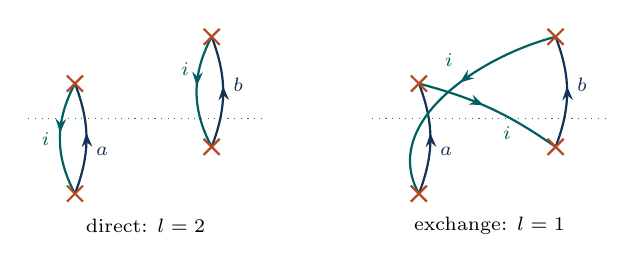
\begin{tikzpicture}[x=1.25cm,y=.78cm,scale=1.12]
  \foreach \shift/\ex in {0/0,3.9/1}{
    \begin{scope}[shift={(\shift,0)}]
    \coordinate (a) at (0,0); \coordinate (b) at (1.55,.85);
    \coordinate (c) at (0,2); \coordinate (d) at (1.55,2.85);
    \draw[pline] (a) to[bend right=21] node[right,dlab,pos=.38] {$a$} (c);
    \draw[pline] (b) to[bend right=21] node[right,dlab,pos=.57] {$b$} (d);
    \ifnum\ex=0
      \draw[hline,teal!75!black] (a) to[bend left=28] node[left,dlab] {$i$} (c);
      \draw[hline,teal!75!black] (b) to[bend left=28] node[left,dlab,pos=.71] {$i$} (d);
      \node[dlab] at (.8,-.58) {direct: $l=2$};
    \else
      \draw[hline,teal!75!black] (a) .. controls (-.45,1.3) and (.7,2.5) .. (d); \node[dlab,teal!75!black] at (.34,2.43) {$i$};
      \draw[hline,teal!75!black] (b) to[bend right=10] node[below,dlab,pos=.37] {$i$} (c);
      \node[dlab] at (.8,-.58) {exchange: $l=1$};
    \fi
    \draw[dotted,teal] (-.53,1.36)--(2.16,1.36);
    \foreach \v in {a,b,c,d}{\node[fvtx] at (\v) {};}
    \end{scope}
  }
\end{tikzpicture}
\end{center}
\[
 D_a=\varepsilon_i-\varepsilon_a,\quad D_b=\varepsilon_i-\varepsilon_b,\qquad
 F=\frac{|\ftil{ai}\ftil{bi}|^2}{D_a(D_a+D_b)D_b}.
\]
Exchanging the upper hole endpoints leaves the numerator and cut energies unchanged. With $h=2$, the signs give $+F-F=0$, as required by $\ann{i}^2=0$. The middle deficit $D_a+D_b$ is a formal line sum.
\end{frame}

\begin{frame}{What happens to the exchange term after regrouping?}
Fix a shared-hole assignment and include the relative time orderings needed for factorisation. Write $U_{\rm P}$ for the unlinked sum with Pauli-allowed overlaps, and $U_{\rm EPV}$ for its formal shared-label extension.
\[
 \underbrace{(U_{\rm P}+U_{\rm EPV})}_{\text{all unlinked pairings}}
 +\underbrace{L_{\rm EPV}}_{\text{linked exchange partners}}
 -\underbrace{(U_{\rm P}+U_{\rm EPV})}_{\text{folded subtraction}}
 =L_{\rm EPV}.
\]
For the pair of contractions just drawn, $L_{\rm EPV}=-U_{\rm EPV}$ after summing matching orders. In the principal term alone, the forbidden occupation has zero net weight. Once the unlinked diagrams cancel against the folded subtraction, the linked exchange contribution remains in the energy.
\begin{block}{How to perform the sums}
Use Pauli-allowed determinants in the original resolvent formula. In the connected diagram formula, sum each line over its full orbital space. A separate veto on coincident labels across different vertices would erase the exchange contribution. Antisymmetry already gives $\vbar{a}{a}{i}{j}=\vbar{a}{b}{i}{i}=0$ at a single vertex.
\end{block}
\end{frame}

\begin{frame}{The two-level benchmark separates the two calculations}
Take one fermion in orbitals $i,a$ with $\Delta=\varepsilon_a-\varepsilon_i>0$, $D=-\Delta$, and off-diagonal mixing $g$. Exact diagonalisation gives
\[
 H=\begin{pmatrix}\varepsilon_i&g^*\\g&\varepsilon_a\end{pmatrix},
 \qquad E_- -\varepsilon_i=
 \frac{\Delta-\sqrt{\Delta^2+4|g|^2}}2
 =-\frac{|g|^2}{\Delta}+\frac{|g|^4}{\Delta^3}+O(|g|^6).
\]
\begin{itemize}
\item \textbf{Determinants.} $QWQ=0$, hence $\av{WR_0WR_0WR_0W}=0$. The folded term gives the entire fourth-order correction
$-E^{(2)}\av{WR_0^2W}=-|g|^4/D^3>0$.
\item \textbf{Wick contractions.} Two simultaneous excursions cannot form a physical state in this one-fermion model. In the unrestricted expansion, the direct and exchange pairings cancel in the principal term. Removing the unlinked sum against the folded term leaves the linked exchange sum with the same coefficient $+|g|^4/\Delta^3$.
\end{itemize}
\end{frame}

\begin{frame}{Counting the two-level diagrams gives the exact coefficient}
For a single virtual orbital, the overlapping ordering creates the same excitation at vertices 1 and 2 and removes it at 3 and 4. The three cut deficits are $D,2D,D$. Before its Wick sign, each pairing has value $F=|g|^4/(2D^3)$.
\begin{center}
\begin{tabular}{lccc}
\toprule
Matching of particles and holes & pairings & loops & signed sum \\
\midrule
Both use the same matching & 2 & 2 & $+2F$ (unlinked) \\
They use opposite matchings & 2 & 1 & $-2F$ (linked) \\
\bottomrule
\end{tabular}
\end{center}
Each species has two possible matchings between the lower and upper vertices. All four have $h=2$. The principal term gives $2F-2F=0$. The folded subtraction cancels $+2F$, leaving
\[
 E^{(4)}=-2F=-\frac{|g|^4}{D^3}=\frac{|g|^4}{\Delta^3}.
\]
Deleting the EPV assignments in the linked sum would incorrectly give zero.
\end{frame}

\begin{frame}{A numerical check: two non-interacting copies}
\numbox{Two non-interacting copies \(A\), \(B\) of a three-level pairing system with one pair each, \(g=0.5\) (cross-copy excitations share no orbital). Restricting the intermediate states of the principal fourth-order term to \((A,AB,B)\), \((A,AB,A)\), \((B,AB,A)\), \((B,AB,B)\): \(-0.00183105\). \(2E^{(2)}_A\langle WR_0^2W\rangle_A\): \(-0.00183105\). \(E^{(4)}_{AB}=0.00109863=2E^{(4)}_A\) to fourteen digits. (\texttt{diagrams.py}, \texttt{fourth\_order\_unlinked}; the \((A,AB,B)\) and \((A,AB,A)\) orderings alone are \(-0.000437\) and \(-0.000478\) -- neither is a product, only their sum is.)}
\begin{itemize}
\item With disjoint orbitals the unperturbed energies add, \(D_{m\otimes n}=D_m+D_n\), and matrix elements and signs factorise; the \((A,AB,B)\) and \((A,AB,A)\) patterns have the denominators of the factorisation identity.
\item Their sum is \(\langle WR_0^2W\rangle_A\,E^{(2)}_B\); the other two give \(E^{(2)}_A\langle WR_0^2W\rangle_B\). The folded term of the two copies, \((E^{(2)}_A+E^{(2)}_B)(\langle WR_0^2W\rangle_A+\langle WR_0^2W\rangle_B)\), has exactly these cross terms: the cross-copy part of \(E^{(4)}\) cancels and \(E^{(4)}_{AB}=E^{(4)}_A+E^{(4)}_B\).
\end{itemize}
\end{frame}

\begin{frame}{Pause to think \#3}
\thinkq{3}{Brillouin-Wigner theory uses \(R_E=Q/(E_0-H_0)\): the \emph{exact} energy in every denominator, and no renormalisation terms at all.
\begin{enumerate}
\item Redo the factorisation identity with \(D_m\to D_m+\Delta E\), \(D_n\to D_n+\Delta E\), \(D_m+D_n\to D_m+D_n+\Delta E\). Does it still factorise?
\item What does this say about the unlinked diagrams of a truncated BW calculation, and about its scaling with system size?
\end{enumerate}}
\end{frame}

\begin{frame}{Answer to pause \#3}
\thinka{%
\begin{enumerate}
\item No. With \(d_m=D_m+\Delta E\) etc.\ the middle denominator is \(D_m+D_n+\Delta E\ne d_m+d_n\) (it is \(d_m+d_n-\Delta E\)), so \(\frac{1}{d_m(d_m+d_n-\Delta E)}\bigl(\frac1{d_n}+\frac1{d_m}\bigr)\ne\frac1{d_m^2d_n}\). The excursion deficits add for disjoint excitations in RS. BW inserts the same global energy shift once in each intermediate-state denominator.
\item The cancellation used in the RS proof fails in general for self-consistent BW truncated at finite order. Spurious cross terms can spoil additivity for two independent copies, as in the week-44 example. The exact energies of two non-interacting copies are additive.
\end{enumerate}}
\end{frame}

\begin{frame}{Consequences for independent systems}
\begin{itemize}
\item \textbf{Additivity at each order.} For $H=H_A+H_B$ on disjoint non-interacting fragments and a product reference, $Z_{AB}=Z_A Z_B$. Thus $\log Z_{AB}=\log Z_A+\log Z_B$ and $E_{AB}^{(n)}=E_A^{(n)}+E_B^{(n)}$. For $M$ identical independent copies the coefficient is $M E_A^{(n)}$.
\item \textbf{Truncated BW.} The global energy in the denominators spoils the RS factorisation identity in general. A finite self-consistent BW truncation can lose size extensivity.
\item \textbf{Summation by topology.} Ladders and rings are families of connected energy graphs. In coupled cluster, products of excitations in $e^T\ket{\ph}$ supply the disconnected open pieces that survive in the wave function.
\end{itemize}
\small The theorem is an order-by-order identity. Convergence of the energy series at a particular coupling is a separate question.
\end{frame}

\begin{frame}{Summary of Thursday}
\footnotesize
\begin{columns}[T]
\column{0.5\textwidth}
\begin{block}{Linked and unlinked}
\begin{itemize}
\item Open diagrams: connected, disconnected-but-linked (products of amplitudes, kept), unlinked (a closed piece floats; removed)
\item Closing all external lines with a vertex joins the open components into an energy graph; detached closed pieces remain unlinked and cancel collectively against the renormalisation terms
\item Normal ordering removes the one-vertex pieces; at fourth order $\frac1{D_m(D_m+D_n)D_n}+\frac1{D_m(D_m+D_n)D_m}=\frac1{D_m^2D_n}$ identifies the unlinked sum cancelled by the folded term
\end{itemize}
\end{block}
\column{0.5\textwidth}
\begin{block}{The theorem}
\begin{itemize}
\item Frantz-Mills: all interleavings of two open histories $\to$ product of denominator products ($S_{rs}$ by induction)
\item $\Delta E=$ connected closed diagrams; $\Psi_0=$ linked diagrams. Proof: $Z(T)=\av{e^{-T(H'-\varepsilon_0)}}$, Dyson series, connected pieces exponentiate, the marked vertex, intervals $\to1/D_k$
\item EPV terms: the exchanged partners of unlinked drawings with coincident labels stay in the linked sum; two-level model: $+|g|^4/\Delta^3$ from them alone
\item Consequences: extensivity ($Z_{AB}=Z_AZ_B$), finite BW can fail, sum by topology $\to$ coupled cluster
\end{itemize}
\end{block}
\end{columns}
\end{frame}


% ======================================================================
\section[Friday 3: Coupled cluster]{Friday, lecture 3: The exponential ansatz}
% ======================================================================

\begin{frame}{Three defects, and one change of ansatz}
\small
\begin{columns}[T]
\column{0.55\textwidth}
\begin{block}{What we have}
\begin{itemize}
\item Truncated CI (chapter 5): variational, \alert{not size consistent} -- CID drops the quadruple that is a product of two doubles
\item Perturbation theory (chapter 9): size extensive, \alert{not variational}, and convergence depends on the partition and coupling
\item RPA (chapter 7): sums rings to all orders, collapses when the mean field goes unstable
\end{itemize}
\end{block}
\column{0.45\textwidth}
\begin{block}{Coupled cluster}
\[
\begin{gathered}\text{CI: }\ \ket{\Psi}=(1+C)\ket{\ph}
\\[5pt]\text{CC: }\ \boxed{\ket{\Psi}=e^{T}\ket{\ph}}\end{gathered}
\]
Size extensive by construction, sums infinite classes of diagrams, a hierarchy of excitation-rank approximations, with polynomial cost at fixed rank. Accuracy need not improve monotonically; the projected energy is not variational.
\end{block}
\end{columns}
\vspace{0.5em}
\small The exponential generates the disconnected products of open components required by the linked-diagram theorem.
\end{frame}

\begin{frame}{The cluster operator}
\small
\[
 T=\sum_{n=1}^{N}T_n,\qquad
 T_n=\frac1{(n!)^2}\sum_{i_1\cdots i_n,a_1\cdots a_n}
 t_{i_1\cdots i_n}^{a_1\cdots a_n}
 a_{a_1}^\dagger\cdots a_{a_n}^\dagger a_{i_n}\cdots a_{i_1}.
\]
The amplitudes are antisymmetric separately in occupied and virtual indices. Thus $T_1$ has prefactor $1$, $T_2$ has $1/4$ and $T_3$ has $1/36$.
\begin{itemize}
\item Pure excitation monomials commute: $[T_m,T_n]=0$. The next frame proves this directly from the fermionic anticommutation relations.
\item On the $N$-particle sector, $T^k=0$ for $k>N$. For $T=T_2$, already $T_2^k=0$ for $2k>N$. The exponential terminates on this sector.
\end{itemize}
\begin{center}
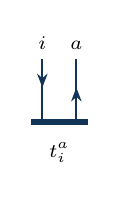
\begin{tikzpicture}[fcidiagram]
  \draw[amp] (-0.5,0) -- (0.5,0);
  \draw[hline] (-0.3,0) -- (-0.3,1.1); \draw[pline] (0.3,0) -- (0.3,1.1);
  \node[dlab,above] at (-0.3,1.1) {$i$}; \node[dlab,above] at (0.3,1.1) {$a$};
  \node[dlab,below] at (0,-0.2) {$t_i^a$};
\end{tikzpicture}
\hspace{3em}
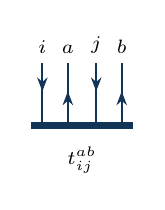
\begin{tikzpicture}[fcidiagram]
  \draw[amp] (-0.9,0) -- (0.9,0);
  \draw[hline] (-0.7,0) -- (-0.7,1.1); \draw[pline] (-0.25,0) -- (-0.25,1.1);
  \draw[hline] (0.25,0) -- (0.25,1.1); \draw[pline] (0.7,0) -- (0.7,1.1);
  \node[dlab,above] at (-0.7,1.1) {$i$}; \node[dlab,above] at (-0.25,1.1) {$a$};
  \node[dlab,above] at (0.25,1.1) {$j$}; \node[dlab,above] at (0.7,1.1) {$b$};
  \node[dlab,below] at (0,-0.2) {$t_{ij}^{ab}$};
\end{tikzpicture}
\par\small The amplitude bars of chapter 5 (week 38): in CC they are the unknowns; every open diagram of yesterday ends on bars like these.
\end{center}
\end{frame}

\begin{frame}{Commuting excitations and the inverse cluster expansion}
Let $X_m$ and $X_n$ be pure excitation monomials of ranks $m,n$. Their single-fermion factors have zero mutual anticommutators: occupied and virtual labels belong to disjoint sets. Moving all $2m$ factors through all $2n$ factors gives
\[
 X_mX_n=(-1)^{(2m)(2n)}X_nX_m=X_nX_m.
\]
If a creation or annihilation label is repeated, both products vanish. Thus $[T_m,T_n]=0$, including overlapping excitations.
\medskip

For a state with nonzero reference overlap, impose intermediate normalisation and write $\ket{\Psi}=(1+C)\ket{\ph}$. The excitation algebra is nilpotent, so
\[
 T=\log(1+C)=C-\tfrac12C^2+\tfrac13C^3-\cdots
\]
is finite on the $N$-particle sector. In particular,
\[
 T_1=C_1,\quad T_2=C_2-\tfrac12C_1^2,\quad
 T_3=C_3-C_1C_2+\tfrac13C_1^3.
\]
Complete CI and complete CC are equivalent when this overlap is nonzero. Truncating $T$ retains products of lower-rank clusters, but omits independent higher-rank clusters.
\end{frame}


\begin{frame}{Why exponentiate at all?}
\small
\[
e^{T}=1+T_1+\Bigl(T_2+\tfrac12T_1^2\Bigr)+\Bigl(T_3+T_1T_2+\tfrac16T_1^3\Bigr)+\Bigl(T_4+T_1T_3+\tfrac12T_2^2+\tfrac12T_1^2T_2+\tfrac1{24}T_1^4\Bigr)+\cdots
\]
Compare with CI, $\ket{\Psi}=(1+C_1+C_2+\cdots)\ket{\ph}$:
\[
C_1=T_1,\qquad C_2=T_2+\tfrac12T_1^2,\qquad C_3=T_3+T_1T_2+\tfrac16T_1^3,\qquad C_4\ni\tfrac12T_2^2 .
\]
\begin{itemize}
\item For nonzero reference overlap, complete $T$ and $C$ are equivalent. Each high-rank CI coefficient is an independent connected cluster plus products of lower-rank clusters. Truncating $T$ drops the independent higher clusters while retaining the products.
\item Truncate $C$ at doubles: the quadruples are gone, and a product of two doubles on separate subsystems \emph{is} a quadruple -- CID is not size consistent (week 38). Truncate $T$ at doubles: $\tfrac12T_2^2$ keeps it, with its amplitude fixed by the doubles.
\item Yesterday, ``disconnected but linked'': $\langle\Phi_{ijkl}^{abcd}|\Psi^{(2)}\rangle=t_mt_n$, a product of first-order doubles. That is $\tfrac12T_2^2$ at lowest order. The exponential generates every disconnected-but-linked diagram from the connected ones, and nothing else -- it is the wave-operator form of the theorem, $\Omega=[\,\cdot\,]_{\rm linked}$, as an ansatz.
\end{itemize}
\end{frame}

\begin{frame}{Pause to think \#4}
\thinkq{3}{Two non-interacting subsystems $A$ and $B$, reference $\ket{\ph}=\ket{\Phi_A}\ket{\Phi_B}$, no amplitude carries indices from both.
\begin{enumerate}
\item Show that $e^{T}\ket{\ph}=\bigl(e^{T_A}\ket{\Phi_A}\bigr)\bigl(e^{T_B}\ket{\Phi_B}\bigr)$. Which property of $T$ is used?
\item Show that $(1+C_2^A+C_2^B)\ket{\ph}$ is \emph{not} a product, and name the missing term.
\item What does 1.\ say about the energy of $A+B$ at any truncation of $T$?
\end{enumerate}}
\end{frame}

\begin{frame}{Answer to pause \#4}
\thinka{%
\begin{enumerate}
\item $T=T_A+T_B$ with $[T_A,T_B]=0$ (they commute: only $\cre{a}\ann{i}$ strings, disjoint orbitals), so $e^{T}=e^{T_A}e^{T_B}$, and since the two act on disjoint orbitals the state factorises.
\item $(1+C_2^A)(1+C_2^B)=1+C_2^A+C_2^B+C_2^AC_2^B$: the cross term is a quadruple excitation, which CID has thrown away. One line, and it is section 5.9 of week 38.
\item The energy of a product state under $H_A+H_B$ is $E_A+E_B$ -- at \emph{any} truncation, because $T_A$ and $T_B$ are truncated independently. Size extensivity is built in; chapter 10 checks it to $10^{-13}$ on three copies of a pairing system.
\end{enumerate}}
\end{frame}

\begin{frame}{Size consistency of the projected CC equations}
For non-interacting fragments with a product reference and a compatible rank truncation, choose $T=T_A+T_B$. Disjoint even operators commute, so
\[
 e^{-T}(H_A+H_B)e^T=\Hbar_A+\Hbar_B.
\]
Reference projection gives $E_{AB}=E_A+E_B$. A projection excited only on $A$ gives
\[
 \mel{\Phi_\mu^A\Phi_B}{\Hbar_A+\Hbar_B}{\Phi_A\Phi_B}
 =\mel{\Phi_\mu^A}{\Hbar_A}{\Phi_A}=0.
\]
For a projection excited on both fragments,
\begin{align*}
\mel{\Phi_\mu^A\Phi_\nu^B}{\Hbar_A+\Hbar_B}{\Phi_A\Phi_B}
={}&\mel{\Phi_\mu^A}{\Hbar_A}{\Phi_A}\braket{\Phi_\nu^B}{\Phi_B}\\
&+\braket{\Phi_\mu^A}{\Phi_A}\mel{\Phi_\nu^B}{\Hbar_B}{\Phi_B}=0.
\end{align*}
The fragment solutions therefore supply a solution of the combined equations with zero connected cross-fragment amplitudes. Select that continuously connected root. Exact additivity for independent fragments is size consistency; for $M$ identical independent fragments it gives linear scaling, or size extensivity.
\end{frame}


\begin{frame}{The similarity transformation and the projected approximation}
For any finite pure-excitation operator $T$, $e^T$ is invertible, with inverse $e^{-T}$. Thus
\[
 \Hbar=e^{-T}He^T,\qquad
 H\ket{E}=E\ket{E}\ \Longrightarrow\
 \Hbar e^{-T}\ket{E}=E e^{-T}\ket{E}.
\]
The full matrices $H$ and $\Hbar$ have the same spectrum, even if $T$ is truncated.
\begin{block}{Exact CC versus truncated CC}
Complete CC chooses $T$ such that $\Hbar\ket{\ph}=E\ket{\ph}$. Truncated CC imposes only selected projections:
\[
 E=\av{\Hbar},\qquad \mel{\Phi_\mu}{\Hbar}{\ph}=0
 \quad(\mu\text{ in the retained excitation space}).
\]
Unretained projections can remain nonzero. The approximation is in the ansatz and the restricted equations, not in the exact similarity identity.
\end{block}
Since $T$ is generally not anti-Hermitian, $e^T$ is nonunitary and $\Hbar$ is generally non-Hermitian. Its left and right eigenvectors differ.
\end{frame}

\begin{frame}{Normal ordering for coupled cluster: $H_N$ versus $W$}
Write the full Hamiltonian as
\[
 H=\Eref+H_N,\qquad
 H_N=\sum_{pq}f_{pq}\no{\cre{p}\ann{q}}
 +\frac14\sum_{pqrs}\as{p}{q}{r}{s}\no{\cre{p}\cre{q}\ann{s}\ann{r}}.
\]
Here $\Eref=\av H$, and $f=h+U$ is the Fock matrix. This is different from Thursday's perturbation:
\[
 H_0=\varepsilon_0+\sum_p\varepsilon_p\no{\cre p\ann p},\qquad
 W=H_I-E^{(1)}I,\qquad
 H_N=\sum_p\varepsilon_p\no{\cre p\ann p}+W.
\]
Consequently, the one-body vertex is $f_{pq}$ in $H_N$, but $\tilde f_{pq}=f_{pq}-\varepsilon_p\delta_{pq}$ in $W$.
\[
 \Hbar=\Eref+\Hbar_N,\qquad \Hbar_N=e^{-T}H_Ne^T,
 \qquad E=\Eref+\av{\Hbar_N}.
\]
For a HF reference $E-\Eref$ is the usual correlation energy; for a general determinant it is simply the energy correction relative to that reference.
\end{frame}


\begin{frame}{Why the BCH series terminates for pure excitations}
\small
Set $K_0=H_N$, $K_{r+1}=[K_r,T]$. Then
\[
 e^{-T}H_Ne^T=\sum_{r\ge0}\frac{K_r}{r!}.
\]
In Wick's theorem there are no contractions between two pure-excitation $T$ vertices. The uncontracted product cancels in a commutator because both strings have even fermion parity. Hence every newly attached $T$ must contract with an operator belonging to the original $H_N$ vertex.
\begin{block}{Count the available operators}
A two-body $H_N$ has at most four fermion operators. Each additional $T$ consumes at least one of them. Therefore $K_5=0$ and
\[
 \boxed{\Hbar_N=H_N+[H_N,T]+\frac{K_2}{2!}+\frac{K_3}{3!}+\frac{K_4}{4!}
 =(H_Ne^T)_c.}
\]
Here $c$ means that every cluster vertex is contracted directly with $H_N$. The fourth commutator can be nonzero; special models can terminate earlier.
\end{block}
For a Hamiltonian with a genuine $k$-body term, the corresponding upper bound is $2k$ commutators.
\end{frame}

\begin{frame}{Termination depends on operator structure}
For unitary CC write $\sigma=T-T^\dagger$. De-excitations introduce contractions between different cluster vertices. Nested commutators can therefore continue without consuming a new operator of the original Hamiltonian each time.
\[
 e^{-\sigma}He^\sigma=H+[H,\sigma]+\tfrac12[[H,\sigma],\sigma]+\cdots
\]
This BCH series does not terminate in general, although special commuting cases can terminate and finite Lie algebras can permit a closed resummation.
\begin{block}{A separate counting argument: the CCD doubles projection}
In $H_NT_2^r$ the two-body term has $4+4r$ fermion operators. To leave four external operators requires $2r$ contractions. All contractions attach to the four operators of $H_N$, so $2r\le4$: only $r=0,1,2$ contribute.
\[
 0=\mel{\Phi_{ij}^{ab}}{(H_N[1+T_2+\tfrac12T_2^2])_c}{\ph}.
\]
Thus the doubles residual is quadratic in $T_2$. The full transformed operator can still contain three- through six-body terms.
\end{block}
\end{frame}


\begin{frame}{The projected equations and the coupled-cluster energy}
For CCSD retain singles and doubles:
\[
 \Delta E=\av{\Hbar_N},\qquad
 \mel{\Phi_i^a}{\Hbar_N}{\ph}=0,\qquad
 \mel{\Phi_{ij}^{ab}}{\Hbar_N}{\ph}=0.
\]
Unretained residuals, including triples and quadruples (and potentially ranks five and six), can remain nonzero. CCD retains only $T_2$ and the doubles equations.
\medskip

The two-body Hamiltonian can remove at most two particle-hole excitations. Hence only $T_1$, $T_2$ and $T_1^2/2$ enter the energy directly:
\[
 \Delta E=\langle H_N(1+T_1+T_2+\tfrac12T_1^2)\rangle_c
 =\sum_{ia}f_{ia}t_i^a+\frac14\sum_{ijab}\as{i}{j}{a}{b}t_{ij}^{ab}
 +\frac12\sum_{ijab}\as{i}{j}{a}{b}t_i^at_j^b.
\]
The $T_1^2$ contraction gives the antisymmetric combination
$\tau_{ij}^{ab}=t_{ij}^{ab}+t_i^at_j^b-t_i^bt_j^a$. In a canonical HF basis $f_{ia}=0$, but correlated singles amplitudes need not vanish: they still affect the doubles equations and the quadratic energy term.
\end{frame}

\begin{frame}{Why the projected CC energy is not an upper bound}
\small
Since $\bra{\ph}e^{-T}=\bra{\ph}$,
\[
 E_{\rm CC}=\mel{\ph}{He^T}{\ph},\qquad
 \braket{\ph}{e^T\ph}=1.
\]
This reference projection differs from the Rayleigh quotient
\[
 E_{\rm var}[T]=\frac{\mel{\ph}{e^{T^\dagger}He^T}{\ph}}
 {\mel{\ph}{e^{T^\dagger}e^T}{\ph}}\ge E_{\rm exact}.
\]
Truncated projected CC does not minimise this quotient, so its energy can lie below the exact ground-state energy. The numerical pairing examples show this directly.
\begin{block}{Left-state information for properties}
A standard stationary CC functional is
\[
 \mathcal L(T,\Lambda)=\mel{\ph}{(1+\Lambda)e^{-T}He^T}{\ph}.
\]
Variation with respect to the de-excitation amplitudes $\Lambda$ gives the right-state residual equations; variation with respect to $T$ determines the left state. Stationarity is not an upper-bound principle.
\end{block}
\end{frame}


% ======================================================================
\section[Friday 4: CCD]{Friday, lecture 4: CCD and the pairing model}
% ======================================================================

\begin{frame}{Deriving the CCD equations: three groups of terms}
\small
$T=T_2$: $\mel{\Phi_{ij}^{ab}}{(H_N[1+T_2+\tfrac12T_2^2])_c}{\ph}=0$ -- the doubles projection with three $T_2$ vertices would require six contractions, but $H_N$ has only four operators. With $P(ij)X_{ij}=X_{ij}-X_{ji}$, $P(ab)X^{ab}=X^{ab}-X^{ba}$, repeated indices summed:
\begin{block}{No $T$: the driving term}
$\mel{\Phi_{ij}^{ab}}{H_N}{\ph}=\as{a}{b}{i}{j}$ (Condon-Slater). It drives the solution connected continuously to $T=0$ at zero interaction.
\end{block}
\begin{block}{One $T$: $H_N$ connected to the amplitude}
\[
P(ab)\,f_{bc}t_{ij}^{ac}-P(ij)\,f_{kj}t_{ik}^{ab}
+\underbrace{\tfrac12\as{a}{b}{c}{d}\,t_{ij}^{cd}}_{\text{pp ladder}}
+\underbrace{\tfrac12\as{k}{l}{i}{j}\,t_{kl}^{ab}}_{\text{hh ladder}}
+\underbrace{P(ij)P(ab)\as{k}{b}{c}{j}\,t_{ik}^{ac}}_{\text{ring}}
\]
$\tfrac12$: two equivalent contractions in each ladder; the ring has inequivalent lines and the full $P(ij)P(ab)$ instead.
\end{block}
\end{frame}

\begin{frame}{Deriving CCD: the four quadratic terms}
\begin{block}{Two $T$'s: both connected to $H_N$ -- only $\as{k}{l}{c}{d}$ can do it}
\[
\tfrac14\as{k}{l}{c}{d}\,t_{ij}^{cd}t_{kl}^{ab}
+\tfrac12P(ij)P(ab)\as{k}{l}{c}{d}\,t_{ik}^{ac}t_{jl}^{bd}
-\tfrac12P(ab)\as{k}{l}{c}{d}\,t_{ij}^{ac}t_{kl}^{bd}
-\tfrac12P(ij)\as{k}{l}{c}{d}\,t_{ik}^{ab}t_{jl}^{cd}
\]
Both amplitudes attach to the same interaction in every term. The last two terms attach three legs from one amplitude and one from the other; there is no detached spectator.
\end{block}

\begin{block}{A useful check on the permutation factor}
Let $X_{ij}^{ab}=\sum_{klcd}\langle kl\Vert cd\rangle t_{ik}^{ac}t_{jl}^{bd}$. Relabelling $k\leftrightarrow l$, $c\leftrightarrow d$ gives $X_{ji}^{ab}=X_{ij}^{ba}$. Hence
\[
 \tfrac12P(ij)P(ab)X_{ij}^{ab}=P(ij)X_{ij}^{ab}=P(ab)X_{ij}^{ab}.
\]
The factor $1/2$ with both permutations is therefore equivalent to using one permutation without $1/2$.
\end{block}
\end{frame}

\begin{frame}{The CCD amplitude equation, and how it is read}
\small
\begin{align*}
D_{ij}^{ab}\,t_{ij}^{ab}={}&\as{a}{b}{i}{j}
+P(ab)f'_{bc}t_{ij}^{ac}-P(ij)f'_{kj}t_{ik}^{ab}
+\tfrac12\as{a}{b}{c}{d}t_{ij}^{cd}+\tfrac12\as{k}{l}{i}{j}t_{kl}^{ab}+P(ij)P(ab)\as{k}{b}{c}{j}t_{ik}^{ac}\\
&+\tfrac14\as{k}{l}{c}{d}t_{ij}^{cd}t_{kl}^{ab}
+\tfrac12P(ij)P(ab)\as{k}{l}{c}{d}t_{ik}^{ac}t_{jl}^{bd}\\
&-\tfrac12P(ab)\as{k}{l}{c}{d}t_{ij}^{ac}t_{kl}^{bd}
-\tfrac12P(ij)\as{k}{l}{c}{d}t_{ik}^{ab}t_{jl}^{cd},
\end{align*}
$D_{ij}^{ab}=f_{ii}+f_{jj}-f_{aa}-f_{bb}$, $f'$ the off-diagonal Fock matrix (zero in a canonical HF basis).
\begin{center}
\begin{tabular}{@{}c@{\hspace{2.5em}}c@{\hspace{2.5em}}c@{\hspace{2.5em}}c@{}}
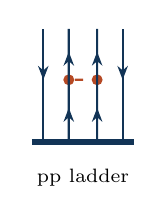
\begin{tikzpicture}[fcidiagram]
  \draw[amp] (-0.9,0) -- (0.9,0);
  \node[vtx] (v1) at (-0.25,1.1) {}; \node[vtx] (v2) at (0.25,1.1) {}; \draw[vint] (v1) -- (v2);
  \draw[hline] (-0.7,0) -- (-0.7,2.0); \draw[hline] (0.7,0) -- (0.7,2.0);
  \draw[pline] (-0.25,0) -- (v1.center); \draw[pline] (0.25,0) -- (v2.center);
  \draw[pline] (v1.center) -- (-0.25,2.0); \draw[pline] (v2.center) -- (0.25,2.0);
  \node[dlab,below] at (0,-0.3) {pp ladder};
\end{tikzpicture}
&
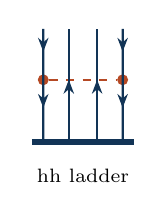
\begin{tikzpicture}[fcidiagram]
  \draw[amp] (-0.9,0) -- (0.9,0);
  \node[vtx] (v1) at (-0.7,1.1) {}; \node[vtx] (v2) at (0.7,1.1) {}; \draw[vint] (v1) -- (v2);
  \draw[pline] (-0.25,0) -- (-0.25,2.0); \draw[pline] (0.25,0) -- (0.25,2.0);
  \draw[hline] (-0.7,0) -- (v1.center); \draw[hline] (0.7,0) -- (v2.center);
  \draw[hline] (v1.center) -- (-0.7,2.0); \draw[hline] (v2.center) -- (0.7,2.0);
  \node[dlab,below] at (0,-0.3) {hh ladder};
\end{tikzpicture}
&
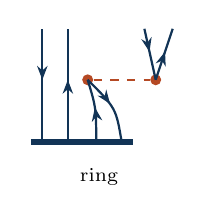
\begin{tikzpicture}[fcidiagram]
  \draw[amp] (-0.9,0) -- (0.9,0);
  \node[vtx] (v1) at (0.1,1.1) {}; \node[vtx] (v2) at (1.3,1.1) {}; \draw[vint] (v1) -- (v2);
  \draw[hline] (-0.7,0) -- (-0.7,2.0); \draw[pline] (-0.25,0) -- (-0.25,2.0);
  \draw[pline] (0.25,0) .. controls (0.25,0.6) .. (v1.center); \draw[hline] (0.7,0) .. controls (0.6,0.6) .. (v1.center);
  \draw[hline] (v2.center) -- (1.1,2.0); \draw[pline] (v2.center) -- (1.6,2.0);
  \node[dlab,below] at (0.3,-0.3) {ring};
\end{tikzpicture}
&
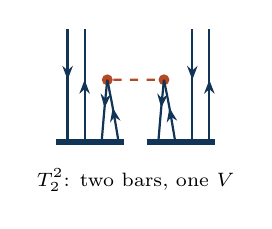
\begin{tikzpicture}[fcidiagram]
  \draw[amp] (-1.3,0) -- (-0.1,0); \draw[amp] (0.3,0) -- (1.5,0);
  \node[vtx] (v1) at (-0.4,1.1) {}; \node[vtx] (v2) at (0.6,1.1) {}; \draw[vint] (v1) -- (v2);
  \draw[hline] (-1.1,0) -- (-1.1,2.0); \draw[pline] (-0.8,0) -- (-0.8,2.0);
  \draw[hline] (-0.5,0) .. controls (-0.45,0.6) .. (v1.center); \draw[pline] (-0.2,0) .. controls (-0.3,0.6) .. (v1.center);
  \draw[hline] (0.5,0) .. controls (0.55,0.6) .. (v2.center); \draw[pline] (0.8,0) .. controls (0.7,0.6) .. (v2.center);
  \draw[hline] (1.1,0) -- (1.1,2.0); \draw[pline] (1.4,0) -- (1.4,2.0);
  \node[dlab,below] at (0.1,-0.3) {$T_2^2$: two bars, one $V$};
\end{tikzpicture}
\end{tabular}
\end{center}
\small Bars at the bottom, $H_N$ on top, four open lines leaving: the third-order diagrams 10, 11, 12 of week 45 with their bottom vertex replaced by an amplitude. Iterating the ladder terms sums ladders to all orders (Brueckner), the ring term sums rings (RPA), the quadratic terms couple them: CCD is a self-consistent combination of both. The last picture is yesterday's disconnected-but-linked quadruple, closed back to a double by one interaction.
\end{frame}

\begin{frame}{Solving CCD: residuals, denominators and the selected root}
Define $R_{ij}^{ab}(t)=\mel{\Phi_{ij}^{ab}}{e^{-T_2}He^{T_2}}{\ph}$ and $D_{ij}^{ab}=f_{ii}+f_{jj}-f_{aa}-f_{bb}$. A Jacobi step is
\[
 t_{ij}^{ab}\leftarrow t_{ij}^{ab}+\frac{R_{ij}^{ab}(t)}{D_{ij}^{ab}},
 \qquad t_{ij}^{ab}(\text{initial})=\frac{\as{a}{b}{i}{j}}{D_{ij}^{ab}}.
\]
\begin{itemize}
\item Check the residual norm, e.g. $\max_{ijab}|R_{ij}^{ab}|<\epsilon_R$, as well as the energy change. A nearly stationary energy alone does not establish an amplitude solution.
\item A nonzero denominator is required for this preconditioner. Small denominators and a poorly conditioned Jacobian can impede convergence.
\item Damping and DIIS can accelerate or stabilise the iteration; neither guarantees convergence or identifies the physical root by itself.
\item Follow the solution continuously from zero interaction, where $T=0$, and check the resulting energy and residuals. Nonlinear CC equations can have several roots.
\end{itemize}
Iteration counts depend on initialisation, damping and stopping tolerances. The following benchmark values are reproduced by solving the projected equations; they do not assume a particular iteration count.
\end{frame}

\begin{frame}{CCD intermediates and computational cost}
With $o$ occupied and $v$ virtual orbitals, a direct four-index inner sum for each amplitude suggests $O(o^4v^4)$ work. Factor the quadratic contractions using
\begin{align*}
 \chi_{kj}&=\tfrac12\as{k}{l}{c}{d}t_{jl}^{cd},&
 \chi_{cb}&=-\tfrac12\as{k}{l}{c}{d}t_{kl}^{bd},\\
 \chi_{klij}&=\tfrac12\as{k}{l}{c}{d}t_{ij}^{cd},&
 \chi_{bkcj}&=\tfrac12\as{k}{l}{c}{d}t_{lj}^{db}.
\end{align*}
The four quadratic terms are then
\[
 \tfrac12\chi_{klij}t_{kl}^{ab}
 +P(ij)P(ab)\chi_{bkcj}t_{ik}^{ac}
 +P(ab)\chi_{cb}t_{ij}^{ac}
 -P(ij)\chi_{kj}t_{ik}^{ab}.
\]
Each intermediate is formed once per iteration. The principal dense contractions scale as
\[
 O(o^2v^4)\quad\text{(pp ladder)},\qquad
 O(o^4v^2)\quad\text{(hh ladder)},\qquad O(o^3v^3)\quad\text{(rings)}.
\]
If $o$ and $v$ grow proportionally to basis size $n$, CCD costs $O(n^6)$ per iteration and stores $O(o^2v^2)$ doubles amplitudes. Full CC, with excitation rank growing with particle number, is not polynomial-cost.
\end{frame}

\begin{frame}{The pairing Hamiltonian and reproducible CCD benchmarks}
Use four doubly degenerate levels, two pairs and spacing $\xi=1$:
\[
 H=\sum_{p=0}^{3}\sum_{\sigma=\pm}p\,n_{p\sigma}
 -G\sum_{pq}P_p^\dagger P_q,\qquad
 G=g/2,\quad P_p^\dagger=a_{p+}^\dagger a_{p-}^\dagger.
\]
The reference occupies levels $0,1$, so $E_{\rm HF}=2-g$. Seniority (number of unpaired fermions) is conserved. On the seniority-zero branch, $T_1=T_3=0$ and CCSD reduces to pair CCD.
\begin{center}
\begin{tabular}{rrrr}
\toprule
$g$ & CCD & FCI & CCD $-$ FCI\\
\midrule
0.25 & 1.73045621 & 1.73045985 & $-3.63\times10^{-6}$\\
0.50 & 1.41663766 & 1.41677428 & $-1.37\times10^{-4}$\\
1.00 & 0.63044275 & 0.63554847 & $-5.11\times10^{-3}$\\
1.50 & $-0.38416526$ & $-0.34819051$ & $-3.60\times10^{-2}$\\
2.00 & $-1.60959440$ & $-1.48965216$ & $-1.20\times10^{-1}$\\
\bottomrule
\end{tabular}
\end{center}
The Fock matrix is diagonal: $f_{i\sigma,i\sigma}=i-G$, $f_{a\sigma,a\sigma}=a$. Mixed-pair particle-hole integrals vanish, so the linear CCD ring term is zero. The pp/hh ladders and the quadratic terms remain.
\end{frame}
\begin{frame}{Reducing CCD to pair amplitudes}
\small
In the seniority-zero space define
\[
 T_2=\sum_{ia}t_i^a P_a^\dagger P_i,\qquad
 S=\sum_{ia}t_i^a,\qquad E=E_{\rm ref}-G S.
\]
Here $i,j$ label occupied \emph{pair levels} and $a,b$ empty pair levels; $t_i^a$ in this frame is a pair amplitude, not a spin-orbital single excitation.
\medskip

The coefficient of a two-pair excitation in $e^{T_2}\ket{\ph}$ is
\[
 C_{ij}^{ab}=t_i^a t_j^b+t_i^b t_j^a\qquad(i\ne j,\ a\ne b).
\]
Pairs commute on disjoint levels, giving the plus sign. Projecting the Schr\"odinger equation on a one-pair excitation gives
\begin{align*}
0={}&-G+2(\epsilon_a-\epsilon_i)t_i^a
 -G\sum_{b\ne a}t_i^b-G\sum_{j\ne i}t_j^a+G S t_i^a\\
 &-G\sum_{j\ne i}\sum_{b\ne a}(t_i^a t_j^b+t_i^b t_j^a).
\end{align*}
The last line couples to the disconnected quadruple. The term $G S t_i^a$ comes from subtracting the correlation energy times the amplitude.
\end{frame}


\begin{frame}{The pairing model: energies and errors}
\begin{center}
\tikzset{every picture/.style={scale=1}}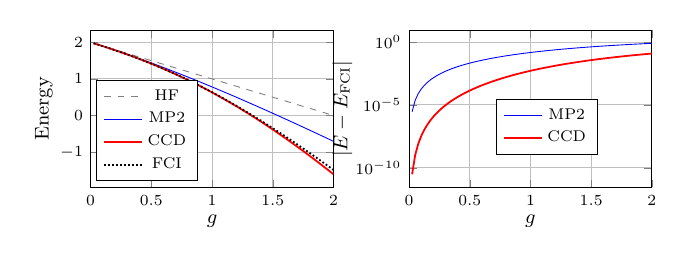
\begin{tikzpicture}[scale=1]
\begin{axis}[name=energy,width=6.4cm,height=4.7cm,xlabel={$g$},ylabel={Energy},xmin=0,xmax=2,grid=major,legend style={font=\scriptsize,at={(.03,.03)},anchor=south west},tick label style={font=\scriptsize},label style={font=\small}]
\addplot[gray,dashed] coordinates {(0.025,1.975) (0.05,1.95) (0.075,1.925) (0.1,1.9) (0.125,1.875) (0.15,1.85) (0.175,1.825) (0.2,1.8) (0.225,1.775) (0.25,1.75) (0.275,1.725) (0.3,1.7) (0.325,1.675) (0.35,1.65) (0.375,1.625) (0.4,1.6) (0.425,1.575) (0.45,1.55) (0.475,1.525) (0.5,1.5) (0.525,1.475) (0.55,1.45) (0.575,1.425) (0.6,1.4) (0.625,1.375) (0.65,1.35) (0.675,1.325) (0.7,1.3) (0.725,1.275) (0.75,1.25) (0.775,1.225) (0.8,1.2) (0.825,1.175) (0.85,1.15) (0.875,1.125) (0.9,1.1) (0.925,1.075) (0.95,1.05) (0.975,1.025) (1,1) (1.025,0.975) (1.05,0.95) (1.075,0.925) (1.1,0.9) (1.125,0.875) (1.15,0.85) (1.175,0.825) (1.2,0.8) (1.225,0.775) (1.25,0.75) (1.275,0.725) (1.3,0.7) (1.325,0.675) (1.35,0.65) (1.375,0.625) (1.4,0.6) (1.425,0.575) (1.45,0.55) (1.475,0.525) (1.5,0.5) (1.525,0.475) (1.55,0.45) (1.575,0.425) (1.6,0.4) (1.625,0.375) (1.65,0.35) (1.675,0.325) (1.7,0.3) (1.725,0.275) (1.75,0.25) (1.775,0.225) (1.8,0.2) (1.825,0.175) (1.85,0.15) (1.875,0.125) (1.9,0.1) (1.925,0.075) (1.95,0.05) (1.975,0.025) (2,0)};\addlegendentry{HF}
\addplot[blue] coordinates {(0.025,1.974819266) (0.05,1.949283174) (0.075,1.923400624) (0.1,1.897180176) (0.125,1.87063007) (0.15,1.843758243) (0.175,1.816572342) (0.2,1.789079737) (0.225,1.761287541) (0.25,1.733202614) (0.275,1.704831583) (0.3,1.676180846) (0.325,1.647256589) (0.35,1.618064791) (0.375,1.588611234) (0.4,1.558901515) (0.425,1.528941051) (0.45,1.498735088) (0.475,1.468288709) (0.5,1.437606838) (0.525,1.40669425) (0.55,1.375555577) (0.575,1.344195313) (0.6,1.312617817) (0.625,1.280827323) (0.65,1.248827943) (0.675,1.216623671) (0.7,1.184218388) (0.725,1.151615867) (0.75,1.118819777) (0.775,1.085833685) (0.8,1.052661064) (0.825,1.019305292) (0.85,0.9857696578) (0.875,0.9520573629) (0.9,0.9181715265) (0.925,0.8841151867) (0.95,0.8498913042) (0.975,0.8155027646) (1,0.780952381) (1.025,0.7462428966) (1.05,0.711376987) (1.075,0.6763572625) (1.1,0.6411862701) (1.125,0.6058664955) (1.15,0.5704003655) (1.175,0.5347902496) (1.2,0.4990384615) (1.225,0.4631472617) (1.25,0.4271188582) (1.275,0.3909554088) (1.3,0.3546590224) (1.325,0.3182317605) (1.35,0.2816756386) (1.375,0.2449926276) (1.4,0.2081846552) (1.425,0.1712536071) (1.45,0.134201328) (1.475,0.09702962329) (1.5,0.05974025974) (1.525,0.0223349668) (1.55,-0.01518456242) (1.575,-0.05281667008) (1.6,-0.09055973266) (1.625,-0.12841216) (1.65,-0.1663723945) (1.675,-0.20443891) (1.7,-0.242610211) (1.725,-0.2808848322) (1.75,-0.3192613371) (1.775,-0.3577383176) (1.8,-0.3963143934) (1.825,-0.4349882108) (1.85,-0.4737584425) (1.875,-0.5126237866) (1.9,-0.5515829661) (1.925,-0.5906347282) (1.95,-0.6297778438) (1.975,-0.6690111067) (2,-0.7083333333)};\addlegendentry{MP2}
\addplot[red,thick] coordinates {(0.025,1.974816404) (0.05,1.949260385) (0.075,1.923324063) (0.1,1.896999532) (0.125,1.870278863) (0.15,1.843154121) (0.175,1.815617377) (0.2,1.787660721) (0.225,1.759276277) (0.25,1.730456214) (0.275,1.701192765) (0.3,1.671478238) (0.325,1.641305034) (0.35,1.610665661) (0.375,1.579552748) (0.4,1.547959064) (0.425,1.51587753) (0.45,1.483301237) (0.475,1.450223458) (0.5,1.416637665) (0.525,1.38253754) (0.55,1.347916992) (0.575,1.312770169) (0.6,1.27709147) (0.625,1.240875556) (0.65,1.204117359) (0.675,1.166812099) (0.7,1.128955282) (0.725,1.09054272) (0.75,1.051570527) (0.775,1.012035133) (0.8,0.9719332842) (0.825,0.9312620494) (0.85,0.8900188215) (0.875,0.84820132) (0.9,0.8058075915) (0.925,0.7628360095) (0.95,0.7192852736) (0.975,0.6751544068) (1,0.6304427536) (1.025,0.5851499753) (1.05,0.5392760461) (1.075,0.4928212476) (1.1,0.4457861632) (1.125,0.3981716715) (1.15,0.3499789392) (1.175,0.3012094141) (1.2,0.2518648167) (1.225,0.201947132) (1.25,0.1514586013) (1.275,0.100401713) (1.3,0.04877919386) (1.325,-0.00340600062) (1.35,-0.05615069517) (1.375,-0.1094515043) (1.4,-0.1633048419) (1.425,-0.2177069303) (1.45,-0.2726538104) (1.475,-0.3281413504) (1.5,-0.3841652556) (1.525,-0.4407210775) (1.55,-0.4978042227) (1.575,-0.5554099624) (1.6,-0.6135334405) (1.625,-0.6721696832) (1.65,-0.7313136067) (1.675,-0.7909600258) (1.7,-0.8511036621) (1.725,-0.9117391518) (1.75,-0.9728610535) (1.775,-1.034463855) (1.8,-1.096541983) (1.825,-1.159089806) (1.85,-1.222101645) (1.875,-1.285571778) (1.9,-1.349494447) (1.925,-1.413863864) (1.95,-1.478674217) (1.975,-1.543919677) (2,-1.6095944)};\addlegendentry{CCD}
\addplot[black,densely dotted,thick] coordinates {(0.025,1.974816404) (0.05,1.949260386) (0.075,1.923324071) (0.1,1.896999565) (0.125,1.870278966) (0.15,1.843154382) (0.175,1.815617953) (0.2,1.787661867) (0.225,1.759278382) (0.25,1.730459846) (0.275,1.701198722) (0.3,1.671487607) (0.325,1.641319259) (0.35,1.610686618) (0.375,1.579582829) (0.4,1.548001271) (0.425,1.515935575) (0.45,1.483379651) (0.475,1.450327709) (0.5,1.416774284) (0.525,1.382714256) (0.55,1.348142868) (0.575,1.313055749) (0.6,1.277448929) (0.625,1.241318857) (0.65,1.204662412) (0.675,1.167476919) (0.7,1.129760156) (0.725,1.091510365) (0.75,1.052726253) (0.775,1.013407002) (0.8,0.973552265) (0.825,0.9331621672) (0.85,0.8922373022) (0.875,0.850778727) (0.9,0.8087879536) (0.925,0.7662669401) (0.95,0.7232180789) (0.975,0.6796441835) (1,0.6355484736) (1.025,0.590934559) (1.05,0.5458064221) (1.075,0.500168399) (1.1,0.4540251604) (1.125,0.4073816912) (1.15,0.3602432696) (1.175,0.3126154463) (1.2,0.2645040232) (1.225,0.2159150315) (1.25,0.1668547112) (1.275,0.1173294894) (1.3,0.06734596005) (1.325,0.01691086348) (1.35,-0.03396893308) (1.375,-0.08528645464) (1.4,-0.1370346367) (1.425,-0.1892063427) (1.45,-0.2417943811) (1.475,-0.2947915206) (1.5,-0.3481905058) (1.525,-0.4019840709) (1.55,-0.4561649532) (1.575,-0.510725905) (1.6,-0.5656597055) (1.625,-0.620959171) (1.65,-0.6766171649) (1.675,-0.7326266062) (1.7,-0.7889804783) (1.725,-0.8456718353) (1.75,-0.9026938096) (1.775,-0.960039617) (1.8,-1.017702562) (1.825,-1.075676044) (1.85,-1.133953559) (1.875,-1.192528703) (1.9,-1.251395177) (1.925,-1.310546788) (1.95,-1.369977453) (1.975,-1.429681197) (2,-1.489652155)};\addlegendentry{FCI}
\end{axis}
\begin{axis}[at={(energy.east)},anchor=west,xshift=1.5cm,width=6.4cm,height=4.7cm,xlabel={$g$},ylabel={$|E-E_{\rm FCI}|$},ymode=log,xmin=0,xmax=2,grid=major,legend style={font=\scriptsize,at={(.97,.03)},anchor=south east},tick label style={font=\scriptsize},label style={font=\small}]
\addplot[blue] coordinates {(0.025,2.861955856e-06) (0.05,2.27886195e-05) (0.075,7.655250605e-05) (0.1,0.0001806103899) (0.125,0.0003511044763) (0.15,0.0006038613368) (0.175,0.0009543887317) (0.2,0.001417870452) (0.225,0.002009159318) (0.25,0.002742768486) (0.275,0.003632861212) (0.3,0.004693239249) (0.325,0.005937330059) (0.35,0.007378173009) (0.375,0.009028404778) (0.4,0.01090024416) (0.425,0.0130054765) (0.45,0.01535543796) (0.475,0.01796099984) (0.5,0.02083255326) (0.525,0.02397999424) (0.55,0.0274127097) (0.575,0.0311395642) (0.6,0.03516888807) (0.625,0.03950846668) (0.65,0.0441655314) (0.675,0.04914675214) (0.7,0.05445823176) (0.725,0.06010550237) (0.75,0.06609352366) (0.775,0.07242668329) (0.8,0.07910879939) (0.825,0.08614312517) (0.85,0.09353235556) (0.875,0.101278636) (0.9,0.1093835729) (0.925,0.1178482466) (0.95,0.1266732253) (0.975,0.1358585811) (1,0.1454039074) (1.025,0.1553083375) (1.05,0.1655705649) (1.075,0.1761888635) (1.1,0.1871611096) (1.125,0.1984848044) (1.15,0.210157096) (1.175,0.2221748033) (1.2,0.2345344384) (1.225,0.2472322301) (1.25,0.2602641469) (1.275,0.2736259193) (1.3,0.2873130623) (1.325,0.301320897) (1.35,0.3156445717) (1.375,0.3302790823) (1.4,0.3452192919) (1.425,0.3604599498) (1.45,0.3759957091) (1.475,0.3918211439) (1.5,0.4079307655) (1.525,0.4243190377) (1.55,0.4409803908) (1.575,0.4579092349) (1.6,0.4750999728) (1.625,0.492547011) (1.65,0.5102447703) (1.675,0.5281876963) (1.7,0.5463702673) (1.725,0.5647870031) (1.75,0.5834324725) (1.775,0.6023012994) (1.8,0.6213881691) (1.825,0.6406878336) (1.85,0.6601951163) (1.875,0.679904916) (1.9,0.6998122106) (1.925,0.7199120602) (1.95,0.7401996094) (1.975,0.7606700899) (2,0.781318822)};\addlegendentry{MP2}
\addplot[red,thick] coordinates {(0.025,3.031774831e-11) (0.05,9.910838816e-10) (0.075,7.686158376e-09) (0.1,3.306869556e-08) (0.125,1.030020358e-07) (0.15,2.615101451e-07) (0.175,5.765141831e-07) (0.2,1.146044301e-06) (0.225,2.104907588e-06) (0.25,3.63178425e-06) (0.275,5.95671481e-06) (0.3,9.36893138e-06) (0.325,1.422497631e-05) (0.35,2.095704167e-05) (0.375,3.008145352e-05) (0.4,4.220721611e-05) (0.425,5.80445229e-05) (0.45,7.841313429e-05) (0.475,0.0001042505164) (0.5,0.0001366196309) (0.525,0.0001767162641) (0.55,0.0002258757828) (0.575,0.0002855792061) (0.6,0.0003574584879) (0.625,0.000443300909) (0.65,0.0005450524877) (0.675,0.0006648203286) (0.7,0.0008048738404) (0.725,0.0009676447691) (0.75,0.001155726008) (0.775,0.001371869159) (0.8,0.001618980852) (0.825,0.001900117808) (0.85,0.002218480717) (0.875,0.002577406926) (0.9,0.002980362052) (0.925,0.003430930544) (0.95,0.00393280533) (0.975,0.004489776613) (1,0.005105719947) (1.025,0.005784583697) (1.05,0.006530376013) (1.075,0.007347151431) (1.1,0.008238997236) (1.125,0.009210019702) (1.15,0.01026433033) (1.175,0.01140603219) (1.2,0.01263920651) (1.225,0.01396789955) (1.25,0.01539610993) (1.275,0.01692777639) (1.3,0.01856676619) (1.325,0.0203168641) (1.35,0.02218176208) (1.375,0.02416504967) (1.4,0.02627020517) (1.425,0.02850058758) (1.45,0.03085942934) (1.475,0.03334982986) (1.5,0.03597474988) (1.525,0.03873700658) (1.55,0.04163926954) (1.575,0.04468405735) (1.6,0.04787373505) (1.625,0.05121051224) (1.65,0.05469644184) (1.675,0.05833341955) (1.7,0.06212318382) (1.725,0.0660673165) (1.75,0.07016724391) (1.775,0.07442423847) (1.8,0.07883942072) (1.825,0.08341376181) (1.85,0.0881480863) (1.875,0.09304307534) (1.9,0.09809927009) (1.925,0.1033170755) (1.95,0.108696764) (1.975,0.1142384802) (2,0.1199422445)};\addlegendentry{CCD}
\end{axis}
\end{tikzpicture}
\end{center}
\small MP2 uses the fixed-Fock partition. CCD over-correlates here. In this seniority-zero, four-particle model the missing independent cluster is $T_4$; $e^{T_2}$ supplies only the disconnected $T_2^2/2$. Including $T_4$ makes this model exact on the ground-state branch. Curves were recomputed from the six pair determinants.
\end{frame}


\begin{frame}{A perturbation parameter for the CCD resummation}
\small
Fix the physical interaction strength $g$, calculate its HF Fock matrix, and define
\[
 H(\lambda)=E_{\rm HF}+F_N+\lambda V_N,\qquad
 F_N=\sum_p f_{pp}\no{\cre p\ann p}.
\]
This is the canonical HF M\o{}ller--Plesset partition. Its denominators $D_{ij}^{ab}=f_{ii}+f_{jj}-f_{aa}-f_{bb}$ are held fixed while expanding in $\lambda$.
\[
 D t(\lambda)=\lambda\{C+L[t(\lambda)]+Q[t(\lambda),t(\lambda)]\},
 \qquad t(\lambda)=\sum_{k\ge1}\lambda^k t^{(k)}.
\]
Consequently,
\[
 Dt^{(1)}=C,\qquad
 Dt^{(k)}=L[t^{(k-1)}]+\sum_{r=1}^{k-2}Q[t^{(r)},t^{(k-1-r)}],
 \quad k\ge2,
\]
\[
 E^{(k+1)}=\frac14\sum_{ijab}\as{i}{j}{a}{b}(t^{(k)})_{ij}^{ab}.
\]
An expansion in physical $g$ about $g=0$ is different: the Fock matrix itself changes with $g$. Specifying the partition is essential when comparing coefficients.
\end{frame}

\begin{frame}{Which perturbative orders does CCD reproduce?}
\small
For a canonical HF reference with a two-body Hamiltonian, $T_2$ starts at first order while correlated singles and connected triples start at second order.
\begin{itemize}
\item The MP2 and MP3 energies involve the first- and second-order doubles amplitudes. CCD reproduces both.
\item At MP4, singles and triples can feed back into doubles and hence the energy. CCD misses these contributions in general. Brillouin's theorem sets $f_{ai}=0$; it does not set all correlated $t_i^a$ to zero.
\item In the pure pairing model, seniority forbids singles and triples. CCD therefore reproduces the complete fourth-order energy. Connected quadruples start at third order and first affect this energy at fifth order.
\end{itemize}
\begin{center}
\begin{tabular}{rrrr}
\toprule
$g$ & order & CCD coefficient & exact RS coefficient\\
\midrule
0.5 & 4 & $-0.0038210766$ & $-0.0038210766$\\
0.5 & 5 & $-0.0006576351$ & $-0.0006043077$\\
1.0 & 4 & $-0.0403096858$ & $-0.0403096858$\\
1.0 & 5 & $-0.0122696366$ & $-0.0112265527$\\
\bottomrule
\end{tabular}
\end{center}
These are coefficients in $\lambda$ for the fixed-Fock partition, evaluated independently in the six-dimensional pair-determinant space.
\end{frame}

\begin{frame}{Resummation, convergence and the choice of partition}
\small
For the pairing model the second-order MP coefficient is
\[
 E_{\rm MP}^{(2)}=-\frac{g^2}{4}\left(\frac1{2+g}+\frac2{4+g}+\frac1{6+g}\right).
\]
At $g=0.5$ it is $-0.0623931624$, whereas the bare one-body partition of week 45 gives $E_{\rm bare}^{(2)}=-7g^2/24=-0.0729166667$.
\medskip

Solving the nonlinear CCD equations at $\lambda=1$ sums the diagram families represented by those equations. Where the Taylor series converges to the same branch, its sum equals this CCD solution; the solution can also exist beyond the Taylor series' convergence disk.
\begin{block}{Two different questions}
Convergence of a finite list of perturbative partial sums does not prove convergence of the infinite series. Convergence of a numerical amplitude iteration concerns a different map and must be checked through its residual.
\end{block}
CCD contains a selected set of connected energy diagrams to all orders, not all connected diagrams of the exact theory. The fifth-order comparison on the previous frame makes the distinction explicit.
\end{frame}


\begin{frame}{Pause to think \#5}
\thinkq{3}{
\begin{enumerate}
\item Yesterday the fourth-order energy was a principal term plus a folded contribution $-E^{(2)}\av{WR_0^2W}$, which cancels the unlinked sum. Where is the folded term in the CCD recursion $D\,t^{(3)}=L[t^{(2)}]+Q[t^{(1)},t^{(1)}]$? (Hint: what does $\mel{\Phi_{ij}^{ab}}{(H_NT_2^2)_c}{\ph}$ contain that $\langle\Phi_{ij}^{ab}|RWRWRW|\ph\rangle$ does not, and the other way round?)
\item A truncated Brillouin-Wigner calculation is not size extensive; a truncated CC calculation is. Both ``resum to all orders''. What is the difference?
\end{enumerate}}
\end{frame}

\begin{frame}{Answer to pause \#5: the subtraction is contained in CC}
For CCD, expand the similarity transform and project on a double. Excitation rank removes the term with $T_2^2$ on the far left:
\[
 R_\mu=\mel{\Phi_\mu}{H_N(1+T_2+\tfrac12T_2^2)}{\ph}
 -t_\mu\,\av{H_NT_2}=0.
\]
Thus the quadratic residual contains the cancellation
\[
 \tfrac12\mel{\Phi_\mu}{H_NT_2^2}{\ph}-t_\mu\Delta E.
\]
In the fixed-Fock perturbation expansion, its third-order amplitude contribution includes $-E^{(2)}t_\mu^{(1)}$. Dividing by $D_\mu$ gives
\[
 -E^{(2)}\frac{V_{\mu0}}{D_\mu^2},
\]
the familiar folded term. The connected residual combines it with the unlinked part of $H_NT_2^2/2$ before evaluating the diagrams.
\small CCD and RS agree at the orders whose complete diagrams CCD contains; they need not agree at higher orders. Truncated BW can spoil additivity through its global energy denominators. CC additivity instead follows directly from the separable exponential and projected equations.
\end{frame}


\begin{frame}{Comparing the methods for the same pairing Hamiltonian}
\small
\begin{block}{The pairing model by every method of the course}
\centering\small\setlength{\tabcolsep}{5pt}
\begin{tabular}{@{}rrrrrrrr@{}}
\toprule
$g$ & HF & MBPT2 & MBPT3 & CID & HF+RPA & CCD & FCI\\
\midrule
0.25 & 1.75000 & 1.73177 & 1.73047 & 1.73051 & 1.71635 & 1.73046 & 1.73046\\
0.50 & 1.50000 & 1.42708 & 1.41667 & 1.41760 & 1.37450 & 1.41664 & 1.41677\\
1.00 & 1.00000 & 0.70833 & 0.62500 & 0.64891 & 0.55459 & 0.63044 & 0.63555\\
1.50 & 0.50000 & $-0.15625$ & $-0.43750$ & $-0.29113$ & $-0.40625$ & $-0.38417$ & $-0.34819$\\
2.00 & 0.00000 & $-1.16667$ & $-1.83333$ & $-1.35209$ & $-1.47622$ & $-1.60959$ & $-1.48965$\\
\bottomrule
\end{tabular}
\end{block}
\begin{itemize}
\item MBPT2 and MBPT3 here use the bare one-body partition of week 45, not the fixed-Fock MP partition used in the preceding coefficient comparison.
\item At $g=2$, HF+RPA is closest to FCI among the displayed approximations. CCD is closest for the other four tabulated couplings. This is a comparison for this model, not a general ranking.
\item HF and CID satisfy variational upper bounds; projected CCD, MBPT and the displayed RPA correction need not. FCI is the exact finite-space result.
\end{itemize}
\small The RPA column uses the particle-hole quasiboson energy $E_{\rm HF}+\tfrac12(\sum_\nu\omega_\nu-\mathrm{Tr}\,A)$. All tabulated CCD, FCI, CID and RPA energies were independently reproduced.
\end{frame}

% ======================================================================
\section{Summary}
% ======================================================================

\begin{frame}{Summary: linked diagrams and Pauli exclusion}
\begin{itemize}
\item Connected open diagrams have one component. Disconnected but linked diagrams have several open components. An unlinked diagram has a detached closed component.
\item Renormalisation terms collectively cancel the unlinked contributions; positive inclusion--exclusion terms are required at higher orders.
\item The energy contains connected closed diagrams. The intermediate-normalised wave function contains linked open diagrams, including disconnected products.
\item The proof uses vacuum exponentiation, cancellation against $Z(T)$ and imaginary-time intervals that yield $1/D_k$. Finite basis, a nondegenerate gap and nonzero reference overlap justify the local perturbative expansion.
\item EPV assignments cancel between Wick pairings before regrouping. Linked exchange contributions can remain after the unlinked/folded cancellation. Do not veto repeated labels separately in a connected-diagram sum.
\item For independent fragments, $Z_{AB}=Z_AZ_B$ proves additivity order by order. Convergence at a chosen coupling is a separate question.
\end{itemize}
\end{frame}

\begin{frame}{Summary: coupled-cluster theory}
\begin{itemize}
\item $e^T$ generates products of connected excitation clusters. With nonzero reference overlap, complete CC and complete CI are equivalent; their truncations differ.
\item Pure excitation operators have no mutual Wick contractions. For a two-body Hamiltonian this makes the BCH series terminate after at most four commutators.
\item The exact similarity transformation preserves the spectrum. Truncated CC solves selected projections and is generally nonvariational; its energy is not a Rayleigh quotient.
\item CCD has a quadratic amplitude equation, $O(n^6)$ dense cost at fixed excitation rank, and factorised fragment solutions. Convergence is checked with residuals.
\item Canonical-HF CCD reproduces MP2 and MP3. For the pure pairing model it also reproduces MP4, but it differs from exact RS at fifth order through the missing connected quadruples.
\item The pairing benchmarks illustrate both the accuracy at weak coupling and the lack of an upper bound at stronger coupling.
\end{itemize}
\end{frame}

\begin{frame}{Next week}
  \begin{exampleblock}{Week 47, November 19--20: coupled cluster continued (chapter 10, sections 10.8--10.12)}
    \small
    Deriving the CCSD equations with intermediates $F_{ae}$, $F_{mi}$, $F_{me}$, $W_{mnij}$, $W_{abef}$, $W_{mbej}$; when singles matter -- the pairing plus particle-hole model on the bare and on the HF reference (Brillouin's theorem visible, CC not invariant under a change of reference); size extensivity verified; beyond CCSD: triples and CCSD(T); a diagrammatic derivation of the amplitude equations from the rules of weeks 45--46; a first look at unitary coupled cluster and why its BCH expansion generally does not terminate.
  \end{exampleblock}
  \vspace{0.5em}
  \small
  Reading: chapter 10, sections 10.8--10.12; Shavitt and Bartlett, chapters 9--10. Code: \texttt{BookPrograms/chapter10/coupledcluster.py}. The week-46 exercises (last frame) are discussed in the exercise session and answered on the week-47 slides.
\end{frame}

% ======================================================================
\section{Answers to the week-45 exercises}
% ======================================================================

\begin{frame}{Exercise 1 a), b): the expansion for arbitrary $\omega$, and the two schemes}
\small
This is exercise 1 of week 44 with $z\to\omega$ and $V\to H_I$; the full answer is on the week-45 slides (and in \texttt{Exercises/AnswersWeek44.tex}). In short:
\begin{itemize}
\item Add and subtract $\omega\ket{\Psi_0}$: $(\omega-H_0)\ket{\Psi_0}=(\omega-E_0+H_I)\ket{\Psi_0}$; multiply by $Q$, invert $\omega-H_0$ on the $Q$ space (possible iff $\omega\ne\varepsilon_n$, $n\ne0$; at $\omega=\varepsilon_0$ this needs the non-degenerate reference), iterate the resulting implicit equation, insert into $E_0-\varepsilon_0=\mel{\ph}{H_I}{\Psi_0}/\braket{\ph}{\Psi_0}$: the overlap cancels and
\[
E_0=\varepsilon_0+\sum_{n=0}^\infty\mel{\ph}{H_I\Bigl(\frac{Q}{\omega-H_0}(\omega-E_0+H_I)\Bigr)^n}{\ph}.
\]
\item $\omega=E_0$ (BW): $\omega-E_0+H_I=H_I$, only interactions and resolvents $Q/(E_0-H_0)$ alternate; implicit, self-consistent, a finite self-consistent truncation is generally not a polynomial in the coupling and can lose size extensivity; its full resummation is exact (Feshbach).
\item $\omega=\varepsilon_0$ (RS): fixed denominators, but $\omega-E_0+H_I=H_I-\Delta E$ must itself be expanded; $E^{(1)}=V_{00}$, $E^{(2)}=\sum V_{0m}V_{m0}/D_m$, $E^{(3)}=\sum V_{0m}V_{mn}V_{n0}/D_mD_n-V_{00}\sum|V_{0m}|^2/D_m^2$. Expanding a BW denominator $1/(D_m+\Delta E)$ reproduces the RS renormalisation term: the two agree term by term through third order; order-truncated RS is polynomial and additive for independent fragments with a separable partition; self-consistent truncated BW need not be.
\end{itemize}
\end{frame}

\begin{frame}{Exercise 1 c): the Hamiltonian in normal-ordered form}
\small
For this exercise $H_I$ is purely two-body ($h_0=h$, so $u=0$). Reference vacuum: the determinant $\ket{\ph}=\prod_{i\le F}\cre{i}\ket{0}$; $\no{\cdots}$ is normal ordering relative to it (week 37: $\cre{a}$, $\ann{i}$ to the left of $\ann{a}$, $\cre{i}$), and $\av{\no{\cdots}}=0$. Wick's theorem for the one-body term, with $\av{\cre{p}\ann{q}}=\delta_{pq}n_p$:
\[
\cre{p}\ann{q}=\no{\cre{p}\ann{q}}+\delta_{pq}n_p
\ \Longrightarrow\
H_0=\sum_{pq}\mel{p}{h_0}{q}\no{\cre{p}\ann{q}}+\sum_i\mel{i}{h_0}{i}.
\]
For the two-body term all contractions are between a creation and an annihilation operator; one contraction gives four terms, two contractions give two:
\begin{align*}
\cre{p}\cre{q}\ann{s}\ann{r}={}&\no{\cre{p}\cre{q}\ann{s}\ann{r}}
+\delta_{pr}n_p\no{\cre{q}\ann{s}}+\delta_{qs}n_q\no{\cre{p}\ann{r}}-\delta_{ps}n_p\no{\cre{q}\ann{r}}-\delta_{qr}n_q\no{\cre{p}\ann{s}}\\
&+\delta_{pr}\delta_{qs}n_pn_q-\delta_{ps}\delta_{qr}n_pn_q .
\end{align*}
\end{frame}

\begin{frame}{Exercise 1 c): collecting the contractions}
\small
Contract with $\tfrac14\vbar{p}{q}{r}{s}$: the four one-body terms are equal by antisymmetry ($\vbar{p}{q}{r}{s}=-\vbar{q}{p}{r}{s}=\ldots$), $4\cdot\tfrac14\sum_{pqi}\vbar{p}{i}{q}{i}\no{\cre{p}\ann{q}}$; the two scalar terms give $2\cdot\tfrac14\sum_{ij}\vbar{i}{j}{i}{j}$:
\[
\boxed{H_I=\frac14\sum_{pqrs}\vbar{p}{q}{r}{s}\no{\cre{p}\cre{q}\ann{s}\ann{r}}+\sum_{pqi}\vbar{p}{i}{q}{i}\no{\cre{p}\ann{q}}+\frac12\sum_{ij}\vbar{i}{j}{i}{j}.}
\]
\begin{itemize}
\item Symbols: $\mel{p}{h_0}{q}$ one-body matrix elements, $\vbar{p}{q}{r}{s}$ antisymmetrised two-body elements, $i,j$ occupied in the reference, $p,q,r,s$ any orbital; the sum of the two scalars is $\Eref=\mel{\ph}{H}{\ph}$, and the one-body parts combine into the Fock operator $f_{pq}=\mel{p}{h_0}{q}+\sum_i\vbar{p}{i}{q}{i}$.
\item Diagrams (week 44, ``the perturbation drawn''): the one-body vertex as a cross with one line in and one out; the two-body vertex as a dashed line with two ends; the mean-field term as a vertex with one line \emph{closed into a bubble} (the hole loop $i$); the scalars as a cross with a closed loop and as two bubbles joined by the interaction.
\end{itemize}
\end{frame}

\begin{frame}{Exercise 1 d): all energy diagrams to second order, with bare vertices}
\small
Reference energy (zeroth and first order) and $E^{(2)}=\sum_m|V_{0m}|^2/D_m$ with $m$ a single or a double:
\begin{center}
\begin{tabular}{@{}c@{\hspace{1.4em}}c@{\hspace{1.4em}}c@{\hspace{1.4em}}c@{\hspace{1.4em}}c@{\hspace{1.4em}}c@{\hspace{1.4em}}c@{}}
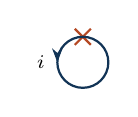
\begin{tikzpicture}[fcidiagram]
  \node[fvtx] (f) at (0,0.9) {}; \draw[hloop] (0.45,0.45) arc (0:360:0.45); \node[dlab,left] at (-0.5,0.45) {$i$};
\end{tikzpicture}
&
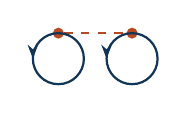
\begin{tikzpicture}[fcidiagram]
  \node[vtx] (v1) at (0,0) {}; \node[vtx] (v2) at (1.3,0) {}; \draw[vint] (v1) -- (v2);
  \draw[hloop] (0,-0.45) ++(0.45,0) arc (0:360:0.45); \draw[hloop] (1.3,-0.45) ++(0.45,0) arc (0:360:0.45);
\end{tikzpicture}
&
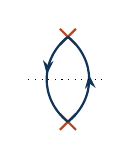
\begin{tikzpicture}[fcidiagram]
  \node[fvtx] (f1) at (0,0) {}; \node[fvtx] (f2) at (0,1.5) {};
  \draw[pline] (f1.center) .. controls (0.5,0.4) and (0.5,1.1) .. (f2.center);
  \draw[hline] (f1.center) .. controls (-0.5,0.4) and (-0.5,1.1) .. (f2.center);
  \draw[dotted] (-0.7,0.75) -- (0.7,0.75);
\end{tikzpicture}
&
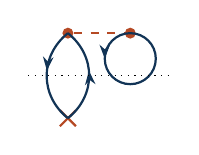
\begin{tikzpicture}[fcidiagram]
  \node[fvtx] (f1) at (0,0) {}; \node[vtx] (t1) at (0,1.5) {}; \node[vtx] (t2) at (1.1,1.5) {}; \draw[vint] (t1) -- (t2);
  \draw[pline] (f1.center) .. controls (0.5,0.4) and (0.5,1.1) .. (t1.center);
  \draw[hline] (f1.center) .. controls (-0.5,0.4) and (-0.5,1.1) .. (t1.center);
  \draw[hloop] (1.1,1.05) ++(0.45,0) arc (0:360:0.45);
  \draw[dotted] (-0.7,0.75) -- (1.8,0.75);
\end{tikzpicture}
&
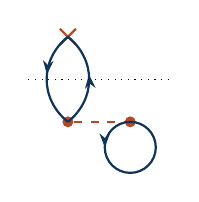
\begin{tikzpicture}[fcidiagram]
  \node[vtx] (b1) at (0,0) {}; \node[vtx] (b2) at (1.1,0) {}; \draw[vint] (b1) -- (b2); \node[fvtx] (f2) at (0,1.5) {};
  \draw[pline] (b1.center) .. controls (0.5,0.4) and (0.5,1.1) .. (f2.center);
  \draw[hline] (b1.center) .. controls (-0.5,0.4) and (-0.5,1.1) .. (f2.center);
  \draw[hloop] (1.1,-0.45) ++(0.45,0) arc (0:360:0.45);
  \draw[dotted] (-0.7,0.75) -- (1.8,0.75);
\end{tikzpicture}
&
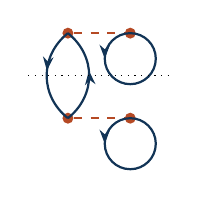
\begin{tikzpicture}[fcidiagram]
  \node[vtx] (b1) at (0,0) {}; \node[vtx] (b2) at (1.1,0) {}; \draw[vint] (b1) -- (b2);
  \node[vtx] (t1) at (0,1.5) {}; \node[vtx] (t2) at (1.1,1.5) {}; \draw[vint] (t1) -- (t2);
  \draw[pline] (b1.center) .. controls (0.5,0.4) and (0.5,1.1) .. (t1.center);
  \draw[hline] (b1.center) .. controls (-0.5,0.4) and (-0.5,1.1) .. (t1.center);
  \draw[hloop] (1.1,-0.45) ++(0.45,0) arc (0:360:0.45); \draw[hloop] (1.1,1.05) ++(0.45,0) arc (0:360:0.45);
  \draw[dotted] (-0.7,0.75) -- (1.8,0.75);
\end{tikzpicture}
&
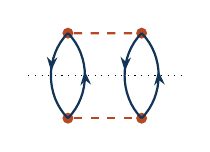
\begin{tikzpicture}[fcidiagram]
  \node[vtx] (b1) at (0,0) {}; \node[vtx] (b2) at (1.3,0) {}; \draw[vint] (b1) -- (b2);
  \node[vtx] (t1) at (0,1.5) {}; \node[vtx] (t2) at (1.3,1.5) {}; \draw[vint] (t1) -- (t2);
  \draw[pline] (b1.center) .. controls (0.4,0.4) and (0.4,1.1) .. (t1.center); \draw[hline] (b1.center) .. controls (-0.4,0.4) and (-0.4,1.1) .. (t1.center);
  \draw[pline] (b2.center) .. controls (1.7,0.4) and (1.7,1.1) .. (t2.center); \draw[hline] (b2.center) .. controls (0.9,0.4) and (0.9,1.1) .. (t2.center);
  \draw[dotted] (-0.7,0.75) -- (2.0,0.75);
\end{tikzpicture}
\\[0.2em]
$\sum_iu_{ii}$ & $\tfrac12\sum_{ij}\vbar{i}{j}{i}{j}$ & $\sum\frac{u_{ia}u_{ai}}{\varepsilon_i-\varepsilon_a}$ & $\sum\frac{U_{ia}u_{ai}}{\varepsilon_i-\varepsilon_a}$ & $\sum\frac{u_{ia}U_{ai}}{\varepsilon_i-\varepsilon_a}$ & $\sum\frac{U_{ia}U_{ai}}{\varepsilon_i-\varepsilon_a}$ & $\tfrac14\sum\frac{|\vbar{a}{b}{i}{j}|^2}{\varepsilon_{ij}^{ab}}$
\end{tabular}
\end{center}
$U_{pq}=\sum_j\vbar{p}{j}{q}{j}$. Rules: sums; $1/D$ per cut (none in first order); $\tfrac12$ per pair of equivalent lines (two pairs in the ring, hence $\tfrac14$; the two-bubble diagram keeps a $\tfrac12$ because exchanging the two ends of the interaction gives the same drawing -- two Wick pairings against the vertex's $\tfrac14$); $(-1)^{h+l}$: every bubble adds one hole line \emph{and} one loop, so all seven are $+$. The four singles diagrams add up to $\sum_{ia}|\tilde f_{ai}|^2/(\varepsilon_i-\varepsilon_a)$, with $\tilde f=u+U$ (and $\tilde f_{ai}=f_{ai}$ for diagonal $h_0$), and vanish in a HF basis; the Hugenholtz form draws each interaction as a dot and merges the direct/exchange pairs.
\end{frame}

\begin{frame}{Exercise 2 e), f): the one-particle system, normal ordered and drawn}
\small
$H_0=\sum_p\varepsilon_p\cre{p}\ann{p}$, $H_I=g\sum_{pq}\cre{p}\ann{q}$, reference $\ket{\ph}=\cre{1}\ket{0}$ (one hole label $i=1$, one particle label $a=2$). From c):
\[
H_0=\varepsilon_1+\sum_p\varepsilon_p\no{\cre{p}\ann{p}},\qquad
H_I=\underbrace{g}_{E^{(1)}=u_{11}}+\;g\sum_{pq}\no{\cre{p}\ann{q}}
=g+g\bigl[\no{\cre{a}\ann{i}}+\no{\cre{i}\ann{a}}+\no{\cre{a}\ann{a}}+\no{\cre{i}\ann{i}}\bigr].
\]
\begin{center}
\begin{tabular}{@{}c@{\hspace{2.5em}}c@{\hspace{2.5em}}c@{\hspace{2.5em}}c@{\hspace{2.5em}}c@{}}
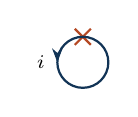
\begin{tikzpicture}[fcidiagram]
  \node[fvtx] (f) at (0,0.9) {}; \draw[hloop] (0.45,0.45) arc (0:360:0.45); \node[dlab,left] at (-0.5,0.45) {$i$};
\end{tikzpicture}
&
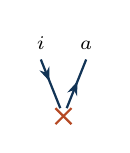
\begin{tikzpicture}[fcidiagram]
  \node[fvtx] (f) at (0,0.5) {}; \draw[hline] (f) -- (-0.4,1.5); \draw[pline] (f) -- (0.4,1.5);
  \node[dlab,above] at (-0.4,1.5) {$i$}; \node[dlab,above] at (0.4,1.5) {$a$};
\end{tikzpicture}
&
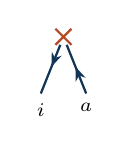
\begin{tikzpicture}[fcidiagram]
  \node[fvtx] (f) at (0,1.0) {}; \draw[hline] (-0.4,0) -- (f); \draw[pline] (0.4,0) -- (f);
  \node[dlab,below] at (-0.4,0) {$i$}; \node[dlab,below] at (0.4,0) {$a$};
\end{tikzpicture}
&
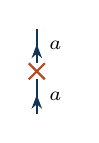
\begin{tikzpicture}[fcidiagram]
  \node[fvtx] (f) at (0,0.75) {}; \draw[pline] (0,0) -- (f); \draw[pline] (f) -- (0,1.5);
  \node[dlab,right] at (0.05,0.3) {$a$}; \node[dlab,right] at (0.05,1.2) {$a$};
\end{tikzpicture}
&
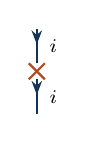
\begin{tikzpicture}[fcidiagram]
  \node[fvtx] (f) at (0,0.75) {}; \draw[hline] (0,0) -- (f); \draw[hline] (f) -- (0,1.5);
  \node[dlab,right] at (0.05,0.3) {$i$}; \node[dlab,right] at (0.05,1.2) {$i$};
\end{tikzpicture}
\\[0.2em]
$g$ (closed) & $g$: creates $\ket{\Phi_i^a}$ & $g$: closes it & $g$ on the particle line & $g$ on the hole line
\end{tabular}
\end{center}
\textbf{f)} In the basis $\{\ket{\ph},\ket{\Phi_i^a}\}$: $\mel{\ph}{H}{\ph}=\varepsilon_1+g$, $\mel{\Phi_i^a}{H}{\Phi_i^a}=\varepsilon_2+g$, off-diagonal $g$:
\[
H=\begin{pmatrix}\varepsilon_1+g&g\\ g&\varepsilon_2+g\end{pmatrix},\qquad
E_-=\varepsilon_1+g+\frac{\Delta}{2}\Bigl(1-\sqrt{1+4g^2/\Delta^2}\Bigr)
=\varepsilon_1+g-\frac{g^2}{\Delta}+0\cdot g^3+\frac{g^4}{\Delta^3}+\bigO{g^6},
\]
$\Delta=\varepsilon_2-\varepsilon_1>0$ -- the first variant of the week-44 benchmark.
\end{frame}

\begin{frame}{Exercise 2 g): third order, drawn}
With $D=\varepsilon_1-\varepsilon_2=-\Delta$ and $V_{00}=V_{mm}=V_{0m}=g$:
\[
E^{(1)}=g,\qquad E^{(2)}=\frac{g^2}{D}=-\frac{g^2}{\Delta},\qquad
E^{(3)}=\frac{V_{0m}V_{mm}V_{m0}}{D^2}-V_{00}\frac{V_{0m}V_{m0}}{D^2}=\frac{g^3}{D^2}-\frac{g^3}{D^2}=0 .
\]
\begin{block}{The diagrams (bare vertex $u_{pq}=g$)}
\begin{itemize}
\item First order: the closed cross, $u_{11}=g$.
\item Second order: cross below, cross above, a particle and a hole line between them, one cut: $u_{ia}u_{ai}/(\varepsilon_i-\varepsilon_a)=-g^2/\Delta$.
\item Third order, \emph{connected}: the cross on the particle line ($+u_{aa}g^2/D^2=+g^3/D^2$, $h=1$, $l=1$) and the cross on the hole line ($-u_{ii}g^2/D^2=-g^3/D^2$, $h=2$, $l=1$): they cancel. \emph{Unlinked}: the closed cross floating between the two cuts, $+V_{00}g^2/D^2$ -- removed by the renormalisation term.
\end{itemize}
\end{block}
\end{frame}

\begin{frame}{Exercise 2 g): cancellation and the fourth-order term}
\begin{block}{Comment}
The principal term $V_{mm}g^2/D^2$ is the sum of three drawings, $u_{aa}-u_{ii}+u_{11}=g-g+g=g$; the renormalisation term is minus the third. The physical answer, $E^{(3)}=0$, comes from the two connected insertions cancelling because $u_{11}=u_{22}$ -- the exact expansion of f) has no $g^3$ term. With normal-ordered vertices ($\ftil{pq}=u_{pq}$ here) the unlinked drawing never appears and $E^{(3)}=\av{WRWRW}=\ftil{aa}g^2/D^2-\ftil{ii}g^2/D^2=0$ directly. Fourth order: $+g^4/\Delta^3$, all of it from the folded term (week 44) -- or, drawn, from the exclusion-principle-violating linked diagrams of Thursday.
\end{block}

\end{frame}

% ======================================================================
\section{Exercises, week 46}
% ======================================================================

\begin{frame}{Exercises week 46}
\small
\begin{enumerate}
\item[1.] \textbf{Linked and unlinked at third order.} Write out all unlinked drawings contained in $\langle\Phi_m|RVRVRV|\ph\rangle$ with bare vertices (pause \#1), evaluate each with the rules, and show that their sum is exactly minus the three displayed groups of renormalisation terms of $\Omega^{(3)}$. Then close every drawing with a top vertex and identify the four pieces of $E^{(4)}$ of week 44.
\item[2.] \textbf{The factorisation theorem.} Prove $S_{rs}=\prod_u A_u^{-1}\prod_v B_v^{-1}$ by induction, and using the boundary condition $S_{0s}=0$ when the closed component finishes before the open component starts, derive the closed-piece form $S_{r-1,s}|_{B_s=0}=\prod_{v<s}B_v^{-1}\prod_{u<r}A_u^{-1}\sum_{j<r}A_j^{-1}$. Check it for $r=3$, $s=2$ by listing the five allowed interleavings, and identify the fifth-order renormalisation terms it corresponds to.
\item[3.] \textbf{Exclusion-principle-violating diagrams.} For the two-level model, list the four complete contractions of the fourth-order diagram with four crosses, their loops and signs, and show that the linked exchange terms alone give $+g^4/\Delta^3$. Redo the count for the pairing model with one pair in two levels: are there EPV terms, and does the answer change?
\end{enumerate}\end{frame}

\begin{frame}{Exercises week 46: coupled cluster}
\small\begin{enumerate}
\item[4.] \textbf{The exponential ansatz} (chapter 10, exercise 1). Prove $[T_m,T_n]=0$; derive $C_1,\dots,C_4$ in terms of $T$'s; show that $e^{T}$ factorises for two non-interacting subsystems while $1+C_2$ does not; explain why the series terminates on an $N$-particle determinant.
\item[5.] \textbf{CCD for the pairing model.} Show that for the pairing interaction the ring term and $t_i^a$ vanish, that the amplitudes can be written as pair amplitudes $t_p^q$ (pair $p$ to pair $q$), and reduce the CCD equation to an equation for the $N_{\rm occ}\times N_{\rm vir}$ matrix $t_p^q$. Solve it by iteration for four levels, two pairs, $g=0.5$, and compare with the table of lecture 4 (\texttt{week46.ipynb} has a general spin-orbital solver to check against).
\end{enumerate}
\small Answers on the week-47 slides.
\end{frame}

\begin{frame}{References and checks for the revised derivations}
\small
\begin{itemize}
\item J. Goldstone, ``Derivation of the Brueckner many-body theory'', \emph{Proc. R. Soc. A} \textbf{239}, 267--279 (1957), \href{https://doi.org/10.1098/rspa.1957.0037}{doi:10.1098/rspa.1957.0037}.
\item I. Shavitt and R. J. Bartlett, \emph{Many-Body Methods in Chemistry and Physics} (Cambridge, 2009), chapters 5--6 and 9.
\item R. J. Bartlett and M. Musia\l{}, ``Coupled-cluster theory in quantum chemistry'', \emph{Rev. Mod. Phys.} \textbf{79}, 291 (2007), \href{https://doi.org/10.1103/RevModPhys.79.291}{doi:10.1103/RevModPhys.79.291}.
\item T. Papenbrock, \href{https://nucleartalent.github.io/ManyBody2018/doc/pub/CCM/html/CCM.html}{The Coupled-Cluster Method}, Nuclear TALENT course notes (2018).
\end{itemize}
\begin{block}{Independent checks for this revision}
The printed CCD residual and energy were compared with exact determinant-space similarity transformations for real and complex test Hamiltonians. The four-commutator BCH identity was also checked. Pair-CCD, FCI, CID and the stated RPA energies were recomputed, and the pairing CCD/RS expansion was compared through fifth order. These tests supplement the algebra; they do not replace it.
\end{block}
\end{frame}
\end{document}
